\chapter{Evaluation}
\label{sec:evaluation}

\section{Effect of Prior Information}

This section will evaluate the application of prior information in a setting where a robot hand moves close to an object and a table. Two sources of depth information will be considered: enhanced stereo matching using IR dot patterns (denoted as \emph{stereo}) and structured light (denoted as \emph{xtion} as in Asus Xtion).

\subsection{Hypotheses}

In the base implementation of the assessed tracking approach, its gradient is mainly determined by the signed distance function. Hence, the optimization is mainly driven by the observation once the iteration is initialized with the reported state. Using additional information that effects the gradient can improve the state estimation by driving it away from distracting observations.

\begin{hypothesis}(Distracting sensor readings)\\
Distracting sensor readings will impair the tracking performance of the manipulator.
\label{hyp:distracting_readings}
\end{hypothesis}

\begin{hypothesis}(Use of prior information)\\
Using prior information will reduce the negative effects of distracting sensor readings. Further, increasing weights will enhance this effect.
\label{hyp:prior_information}
\end{hypothesis}


\subsection{Setup}

A robot is placed in front of a table with a bottle on it. The left hand is moving from close to the table plane towards the object. Once the object is pushed, the hand moves up and back to its initial position.
\Cref{fig:prior_setting} shows the setup with stereo depth and reported robot configuration at the initial state.
The motion sequence is divided into 5 states which change by 4 movements. The movement phases are defined in \cref{tab:prior_movement_phases}. The first three states and the final state are shown in \cref{fig:prior_movement_phases}.
Especially the movement phases 2 and 4, respectively movements starting in states shown in \cref{fig:prior_movement_phases_start,fig:prior_movement_phases_start} are of interest.

\begin{figure}
\centering
\begin{minipage}{0.45\textwidth}
\centering
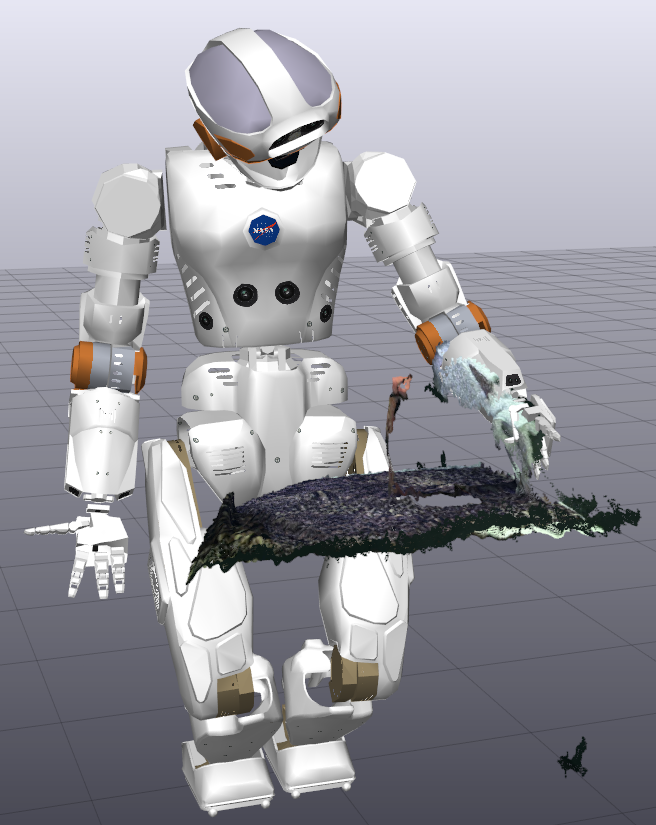
\includegraphics[width=1.0\textwidth]{images/eval_prior/sequence/prior_setting.png} 
\caption{Joint prior setup}
\label{fig:prior_setting}
\end{minipage}
%
\hspace{0.3cm}
\begin{minipage}{0.45\textwidth}
\vspace{0.8cm}
\centering
\subfloat[start (t=0)]{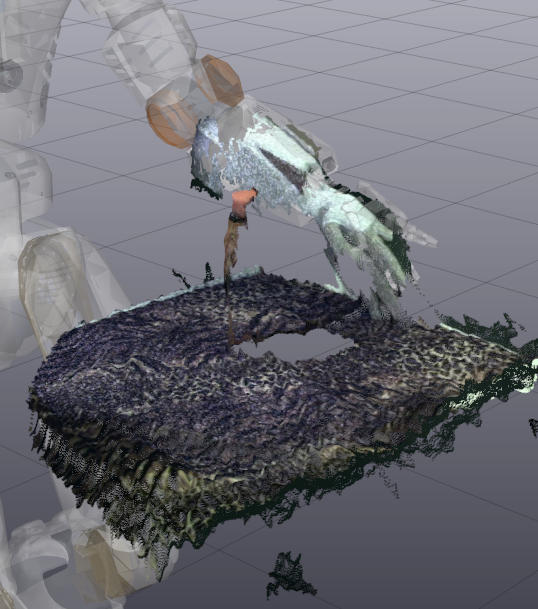
\includegraphics[width=0.5\textwidth]{images/eval_prior/sequence/bottle_0_init.png} \label{fig:prior_movement_phases_start}}
\subfloat[moved upwards (t=10)]{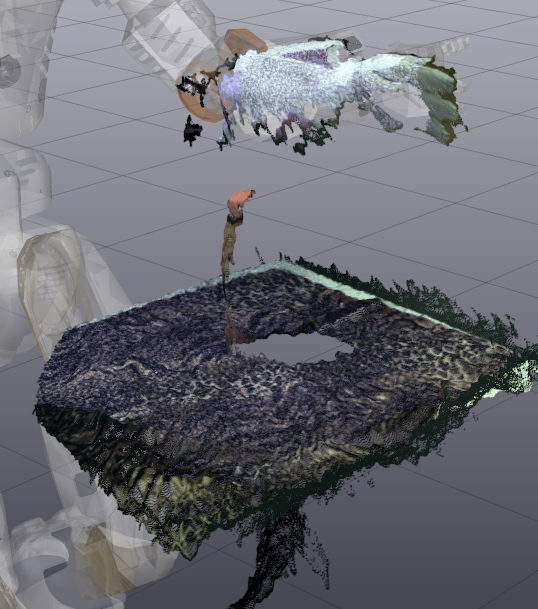
\includegraphics[width=0.5\textwidth]{images/eval_prior/sequence/bottle_10_up.png} }

\subfloat[object contact (t=22)]{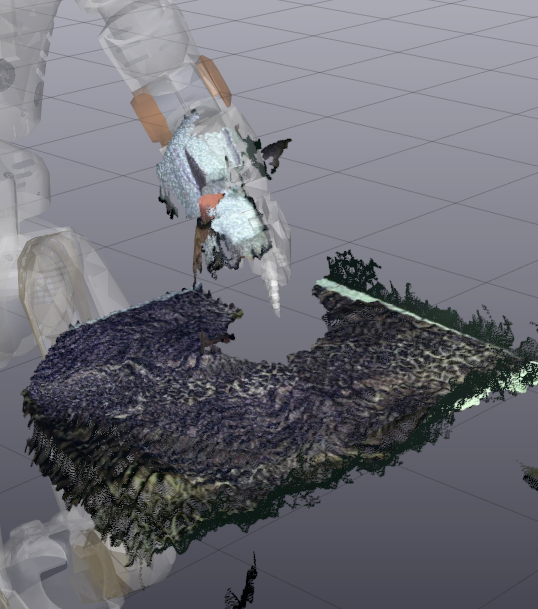
\includegraphics[width=0.5\textwidth]{images/eval_prior/sequence/bottle_22_object.png} 
\label{fig:prior_movement_phases_contact}}
\subfloat[end (t=35)]{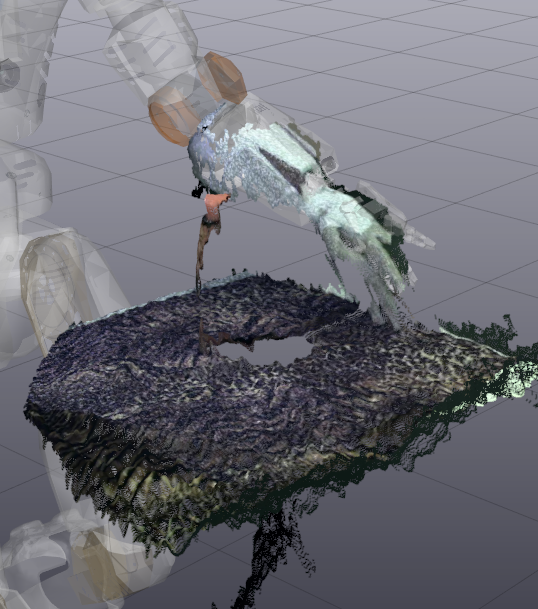
\includegraphics[width=0.5\textwidth]{images/eval_prior/sequence/bottle_35_end.png} }
\caption{Sequence of states between movements}
\label{fig:prior_movement_phases}
\end{minipage}
\end{figure}

\begin{table}
\centering
\begin{tabular}{|c|l|l|}
\hline
 & \emph{time (s)} & \emph{movement description} \\
\hline
1 & 0$\dots$3 & arm resting on table \\
\hline
2 & 3$\dots$10 & upward from table \\
\hline
3 & 10$\dots$20 & towards object \\
\hline
4 & 20$\dots$30 & away from object \\
\hline
5 & 30$\dots$35 & downward towards table \\
\hline
\end{tabular}
\caption{Phases of arm movement}
\label{tab:prior_movement_phases}
\end{table}

During the movement, depth data is collected simultaneously from the MultiSense stereo sensor and the Asus Xtion structured light sensor. Hence, the stereo feature matching benefits from the distinctive IR dots.

\subsection{Results}
\label{sec:prior_results}

The error in joint and task space is computed as L2 norm (Euclidean distance) of its components and plotted over time. In joint space these components are the left fingers (13 DoF: 3 \emph{leftIndexFingerPitch}, 3 \emph{leftMiddleFingerPitch}, 3 \emph{leftPinkyPitch}, 3 \emph{leftThumbPitch} and 1 \emph{leftThumbRoll}) and the left arm (7 DoF: \emph{leftShoulderPitch/Roll/Yaw}, \emph{leftElbowPitch}, \emph{leftForearmYaw}, \emph{leftWristRoll/Pitch}). In task space, the 3D position ($x,y,z$) and the 3D orientation (\textit{roll}, \textit{pitch}, \textit{yaw}) of the left hand (frame: \emph{leftPalm}) are computed via forward kinematics on the reported and estimated robot configuration.

\subsubsection{Common Weight}

The plots compare the joint and task space errors for the two depth sources for common weights in the range 0 to 5. The common weighting scheme \emph{Weighted L2 norm of joint position deviation} (objective function \cref{eqn:objf_weightedL2}) is applied. A weight of 0 indicates that no prior is used at all.

\paragraph{Stereo}

\Cref{fig:stereo_joint_error} compares the joint error for left fingers and arm. For both parts, after the optimization reaches the steady state, the maximum error is reached when no prior information from the reported configuration is used. In this case, the configuration is solely optimized using the distance to the observed point cloud. If the manipulator is close to a large concentration of points, it will get dragged into it (\cref{fig:no_prior_fingers_table}).
The general trend is that the error decreases with increasing prior weight. This is not true for the arm movement in the second half of phase 4 ($t=[20,30]$), where weights of $0.2$ and $0.5$ result in larger errors than using no prior.

The largest decrease in error can be seen for the finger joints when using already a small weight of $0.2$. A similar effect is not present for the arm joints. This is presumably because the robot can only observe the lower part of its arm and hence the arm configuration is mostly determined by its initial state close to the reported state.

\begin{figure}
\captionsetup{width=0.5\textwidth}
\centering
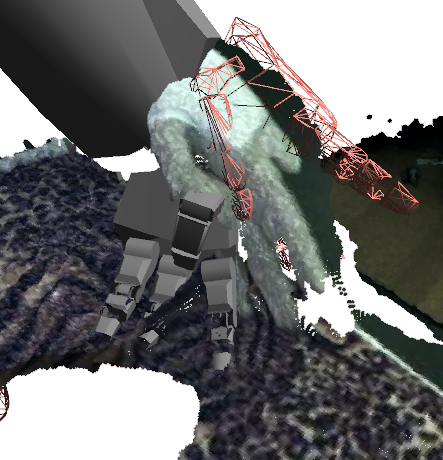
\includegraphics[width=0.5\textwidth]{images/eval_prior/fingers_in_table.png}
\caption[Wrong association of data points]{Association of unrelated points to the robot hand. Fingers get dragged into nearby concentration of points when solely using the signed distance function as objective}
\label{fig:no_prior_fingers_table}
\end{figure}

\begin{figure}
\centering
\subfloat[finger joints]{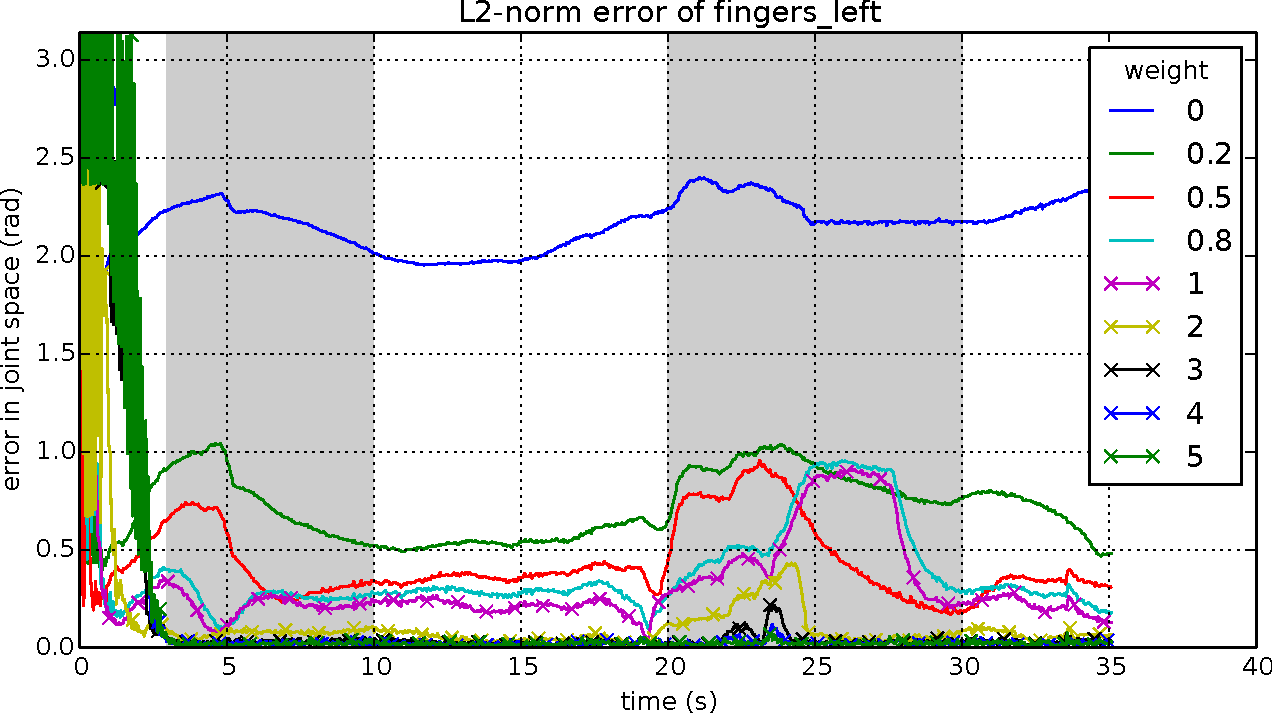
\includegraphics[width=0.5\textwidth]{images/eval_prior/common_weights/stereo_finger_joint_error.pdf} \label{fig:stereo_joint_error_hand} }
%
\subfloat[arm joints]{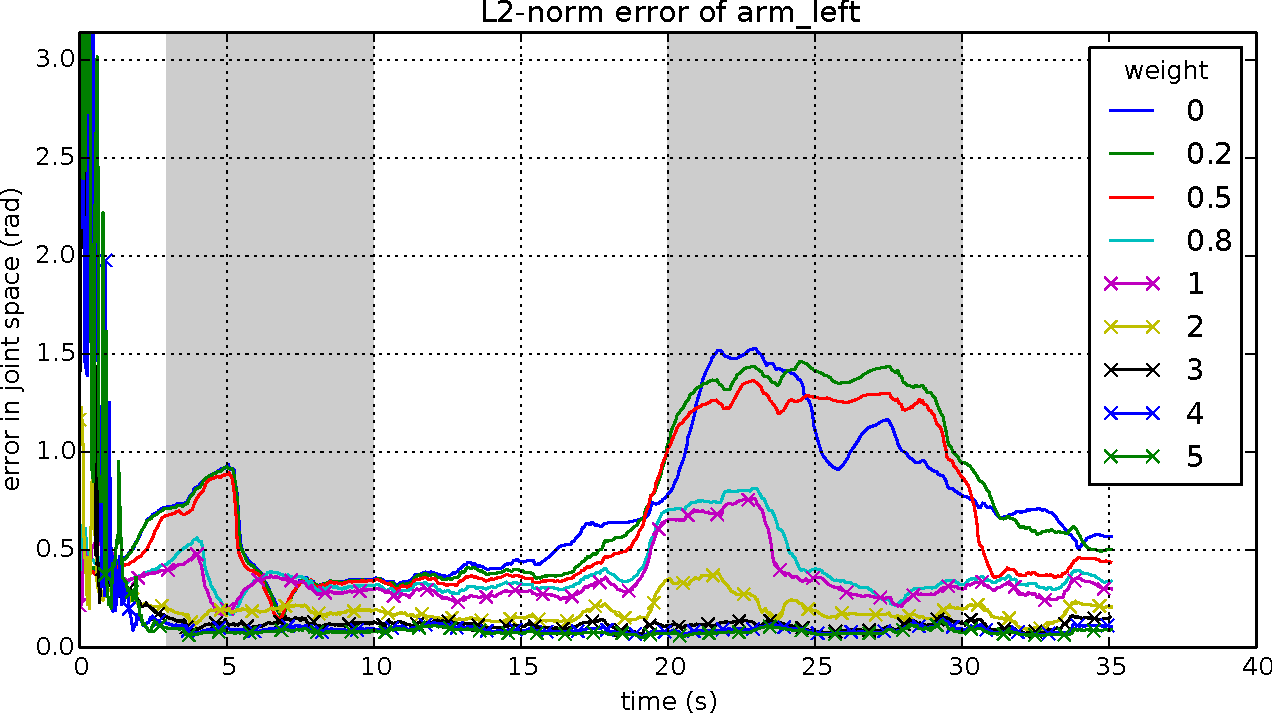
\includegraphics[width=0.5\textwidth]{images/eval_prior/common_weights/stereo_arm_joint_error.pdf} \label{fig:stereo_joint_error_arm} }
\caption[]{Stereo, joint space error for left finger and arm joints}
\label{fig:stereo_joint_error}
\end{figure}

As the hand position and orientation only depends on the arm configuration but not the finger configuration, we expect some relation between the joint error of the arm and the pose error on the hand frame. We can see this relation, when comparing the joint space error for the arm in \cref{fig:stereo_joint_error_arm} and the hand pose error in \cref{fig:stereo_hand_pose_error}. In particular the error increases in phases where the hand moves upwards and when it moves away from the object. The position error can be reduced significantly when using a prior with low weight ($0.2$), where as the orientation error reduces only when using prior weights larger or equal than $0.8$.

\begin{figure}
\centering
\subfloat[position error]{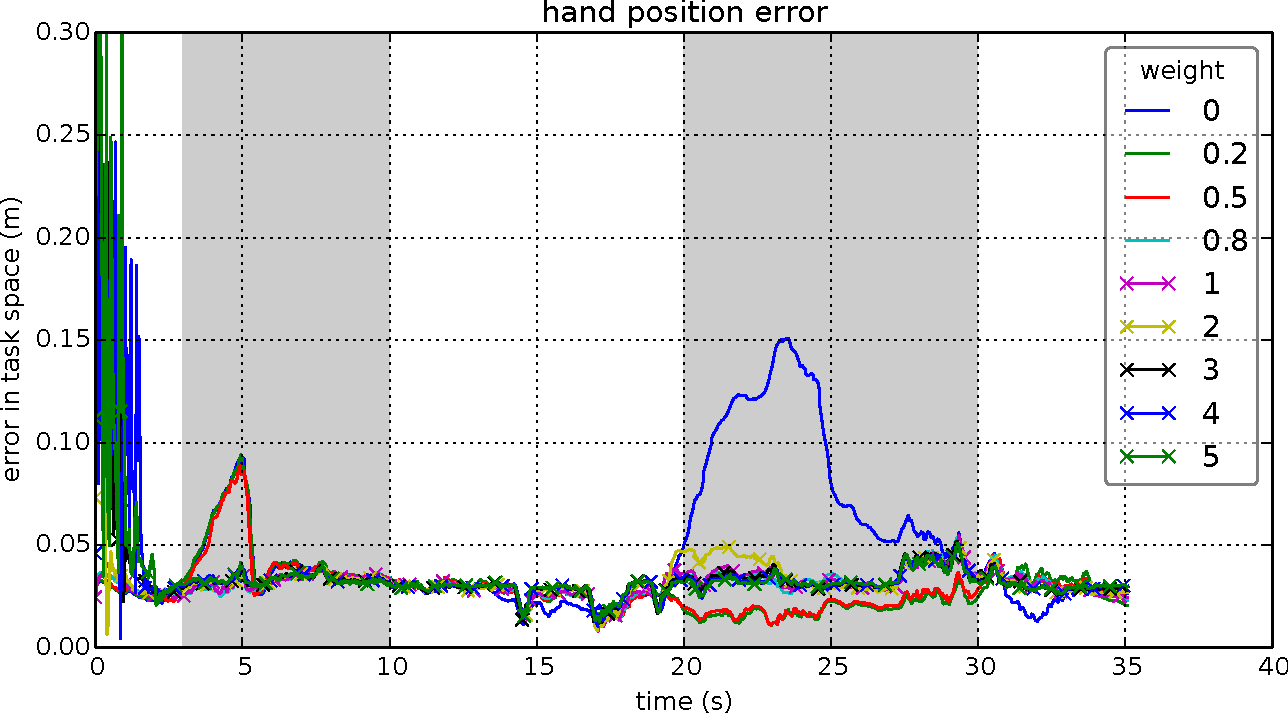
\includegraphics[width=0.5\textwidth]{images/eval_prior/common_weights/stereo_hand_pos_error.pdf} \label{fig:stereo_hand_pos_error}}
%
\subfloat[orientation error]{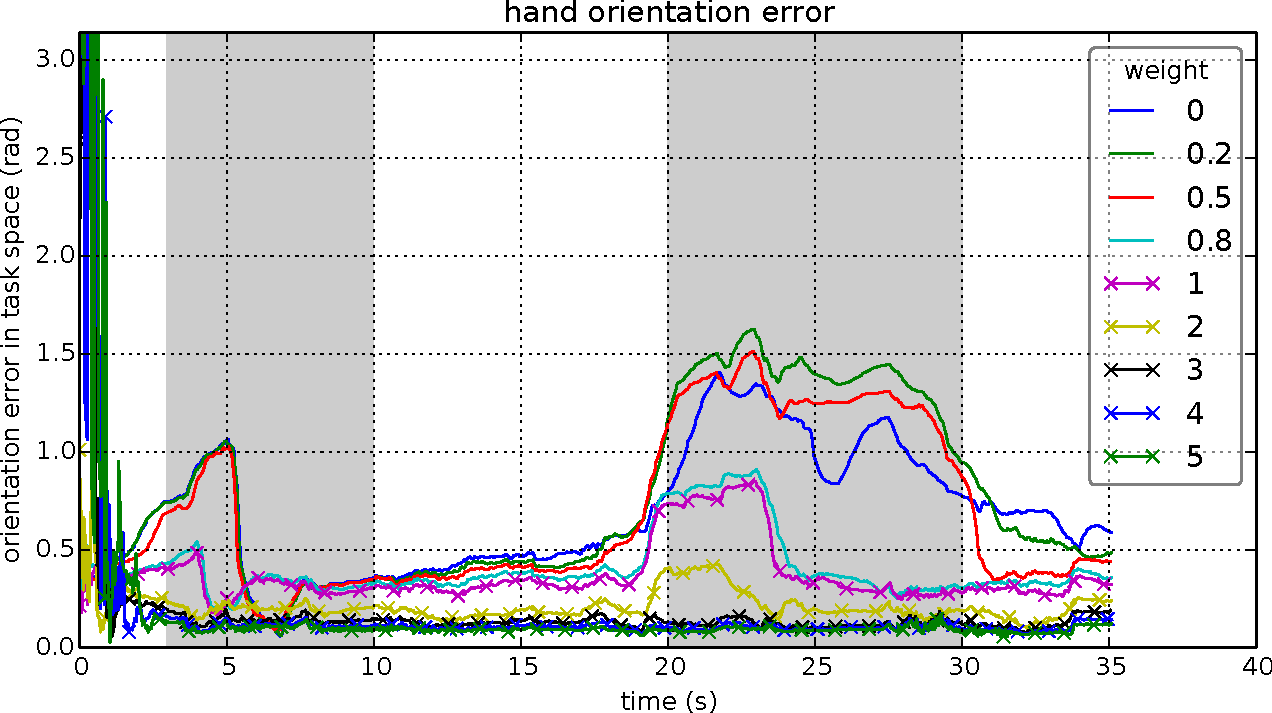
\includegraphics[width=0.5\textwidth]{images/eval_prior/common_weights/stereo_hand_ori_error.pdf}
\label{fig:stereo_hand_ori_error}}
\caption{Stereo, task space error for left hand pose}
\label{fig:stereo_hand_pose_error}
\end{figure}



\paragraph{Asus Xtion}

Using the structured light sensor Asus Xtion, the behaviour of decreasing error with increasing weight is comparable to that one saw for the stereo matching sensor. Similar to the stereo sensor (\cref{fig:stereo_joint_error_hand}), the error on the finger joints reduces significantly when already using a small weight of $0.2$ (\cref{fig:xtion_joint_error_hand}).
In contrast to small the error on the arm joints when using stereo in the phase of moving towards the object (\cref{fig:stereo_joint_error_arm}), the error in this phase when using the Xtion sensor is fairly large for no and low weighted prior (\cref{fig:xtion_joint_error_arm}).

\begin{figure}
\centering
\subfloat[finger joints]{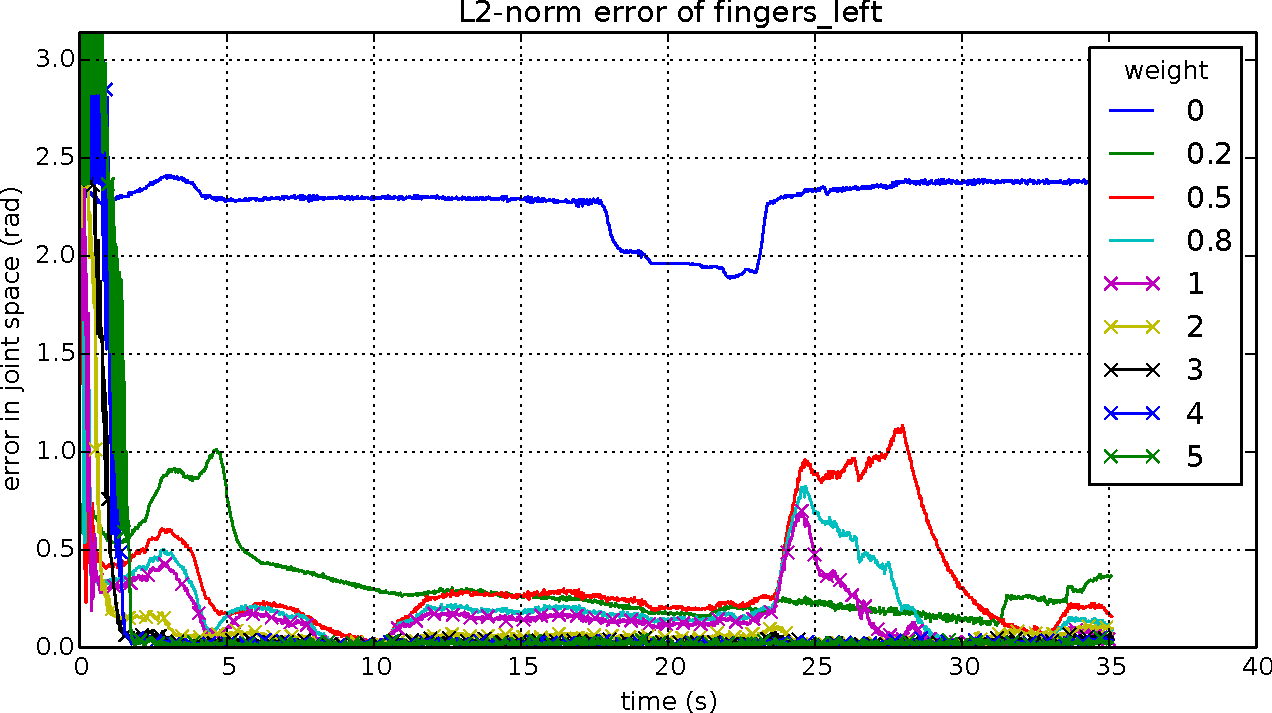
\includegraphics[width=0.5\textwidth]{images/eval_prior/common_weights/xtion_finger_joint_error.pdf} \label{fig:xtion_joint_error_hand}}
%
\subfloat[arm joints]{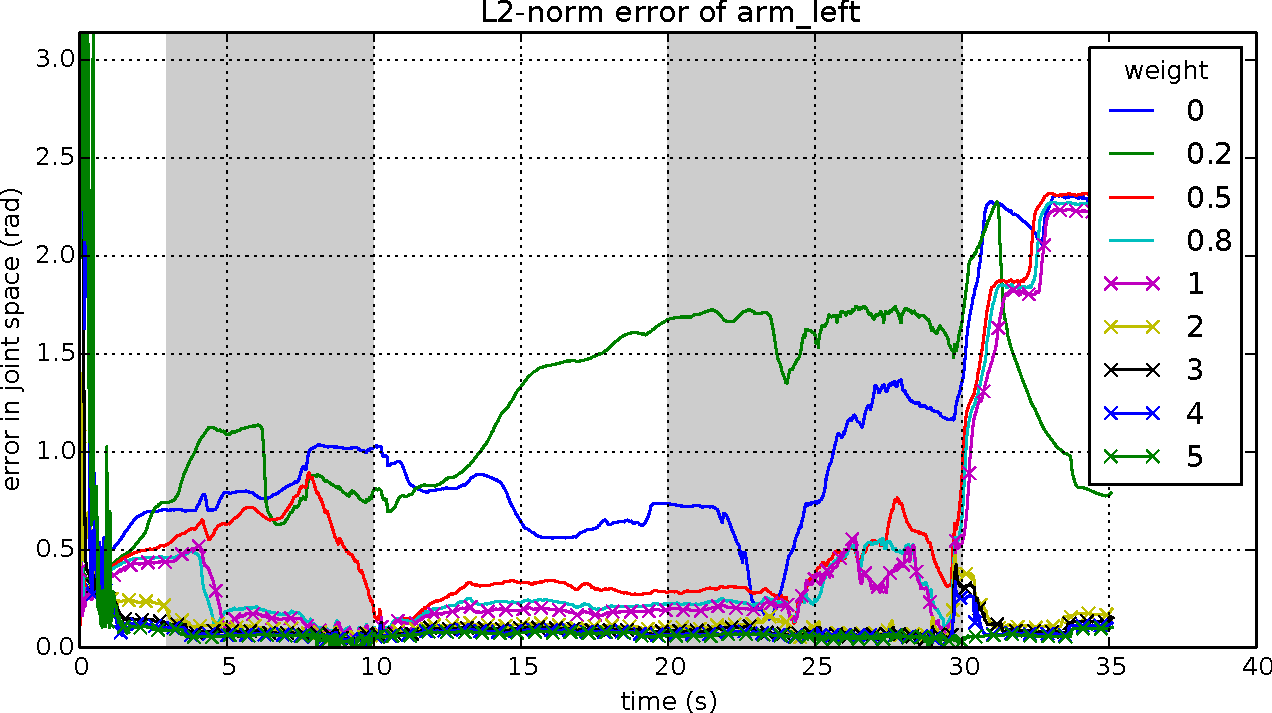
\includegraphics[width=0.5\textwidth]{images/eval_prior/common_weights/xtion_arm_joint_error.pdf} \label{fig:xtion_joint_error_arm}}
\caption{Xtion, joint space error for left finger and arm joints}
\label{fig:xtion_joint_error}
\end{figure}

As before, the hand pose error is only effected by the arm joint errors and thus the hand position error shown in \cref{fig:xtion_hand_pos_error} is large in the same moving phase towards the object. For using the structured light sensor, a common weight of at least $2$ is required to drive the solution towards the reported hand position.

\begin{figure}
\centering
\subfloat[position error]{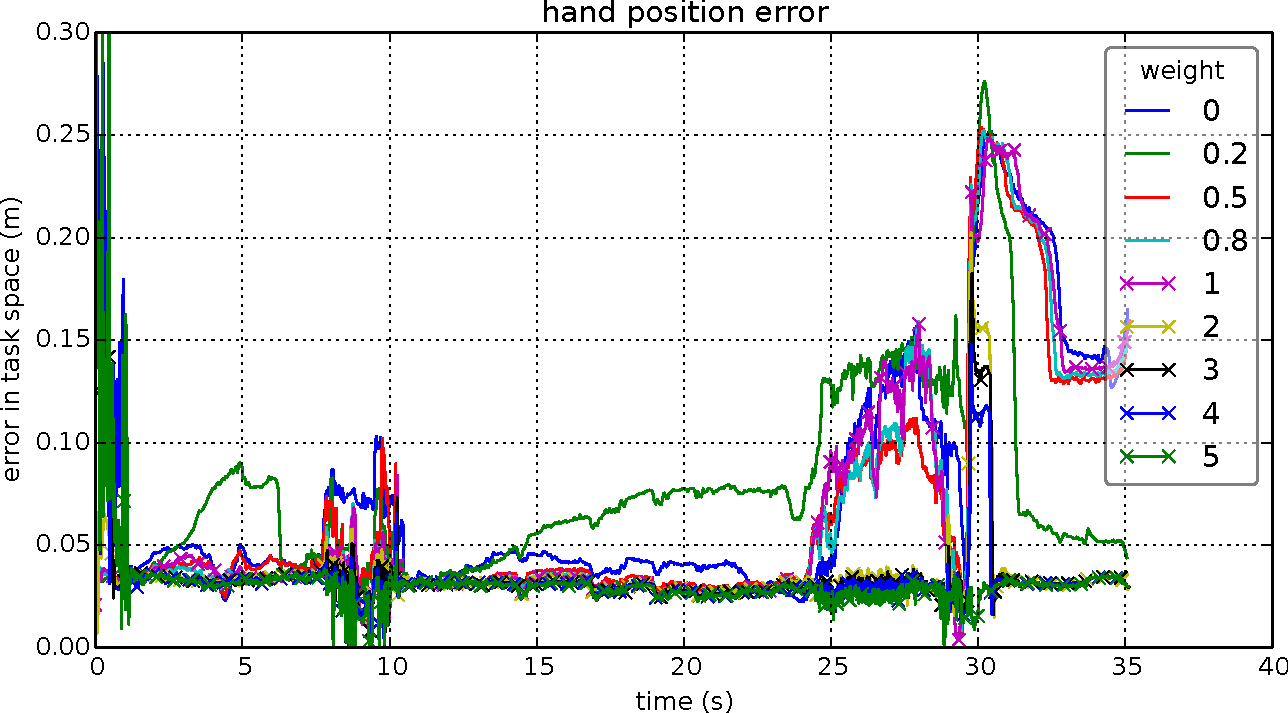
\includegraphics[width=0.5\textwidth]{images/eval_prior/common_weights/xtion_hand_pos_error.pdf} \label{fig:xtion_hand_pos_error}}
%
\subfloat[orientation error]{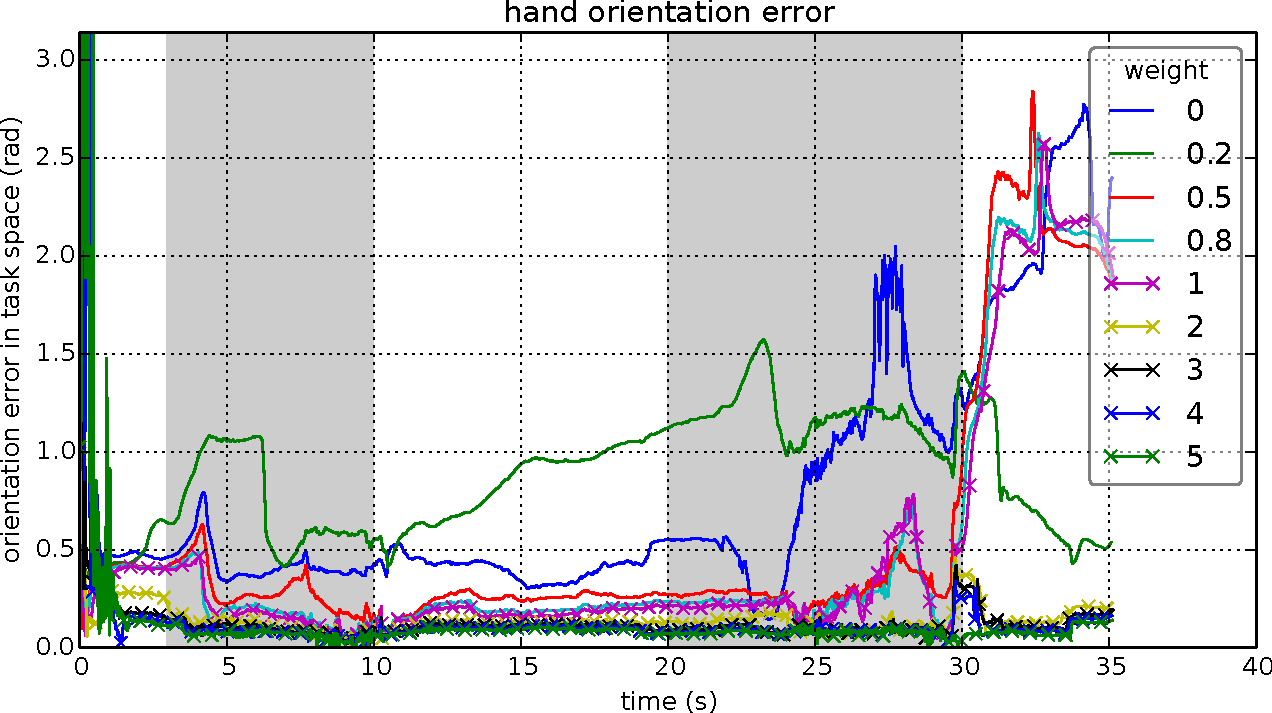
\includegraphics[width=0.5\textwidth]{images/eval_prior/common_weights/xtion_hand_ori_error.pdf} \label{fig:xtion_hand_ori_error}}
\caption{Xtion, task space error for left hand pose}
\label{fig:xtion_hand_pose_error}
\end{figure}

\subsubsection{Individual Weights}

Individual weighting is applied to stereo depth data only. This weighting scheme enables to weight each combination of joint derivations separately as defined by \cref{eqn:objf_indiv_weighted}. For simplicity, only single joint deviations are weighted. That is, the weight matrix $Q$ will be a diagonal matrix where only the diagonal elements $q_{i,i}$ will be changed.

In this scenario, three setting of joints are weighted and this scheme is captured in the legend as follows: first, all diagonal elements of $Q$ are set to the weight \emph{q}, second, the 13 finger joints are set to the weight \emph{fingers} and optionally third, the two palm joints (leftWristRoll, leftWristPitch) are set to the value \emph{parm}. E.g., a plot named \texttt{q 1, fingers 0.2, palm 5} indicates that finger joints in the diagonal are weighted by $0.2$, palm joints are weighted with $5$ and the remaining joints are weighted with $1$.

\Cref{fig:indiv_joint_error} shows again the joint space error for fingers and arms separately. From these plots we can see that the individual weighting affects the fingers and the arm in different ways. The finger joint error in \cref{fig:indiv_joint_error_hand} shows that, raising the palm weights and keeping the remaining constant actually impairs the performance (e.g., compare constant \texttt{q 1, fingers 0.2} and palm weights raised to \texttt{palm 5}). In contrast to this, the arm joint error is reduced when increasing the palm weights and keeping remaining weights constant (e.g., compare constant \texttt{q 0.2, fingers 0.2, palm 5} and palm weights raised to \texttt{q 0.2, fingers 0.2, palm 25}).

\begin{figure}
\centering
\subfloat[finger joints]{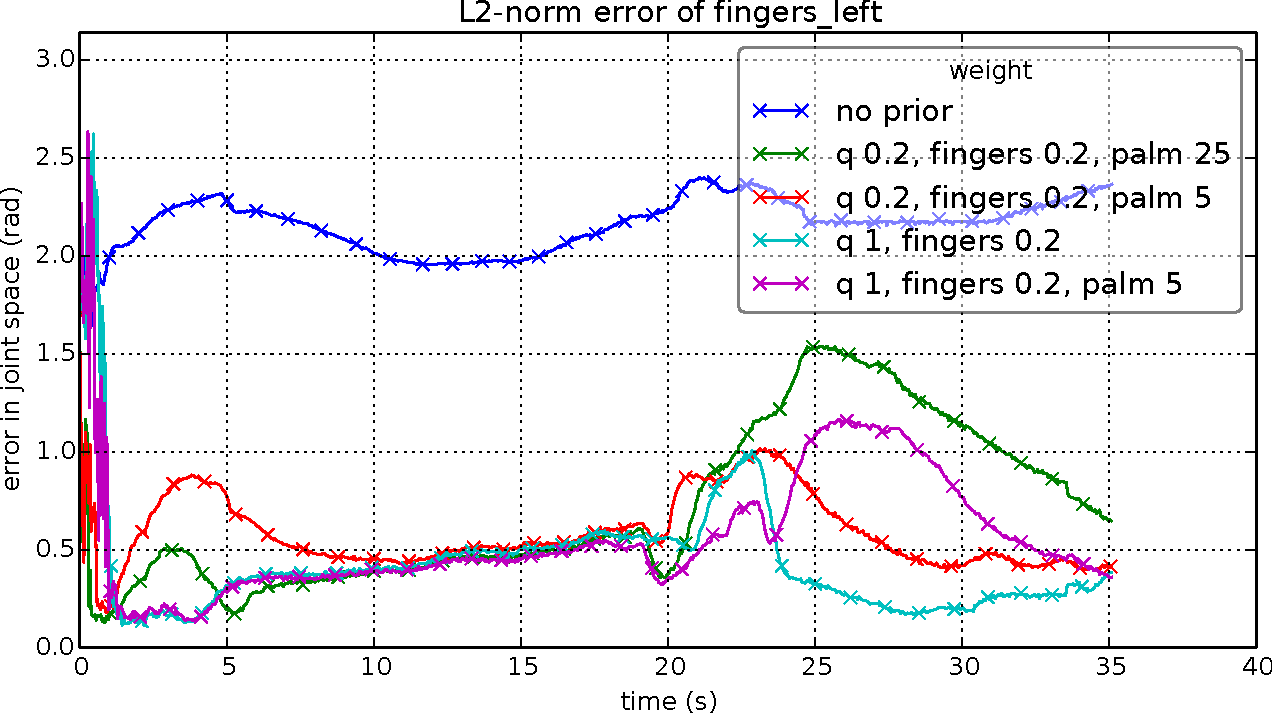
\includegraphics[width=0.5\textwidth]{images/eval_prior/inidv_weights/stereo_finger_joint_error.pdf} \label{fig:indiv_joint_error_hand}}
%
\subfloat[arm joints]{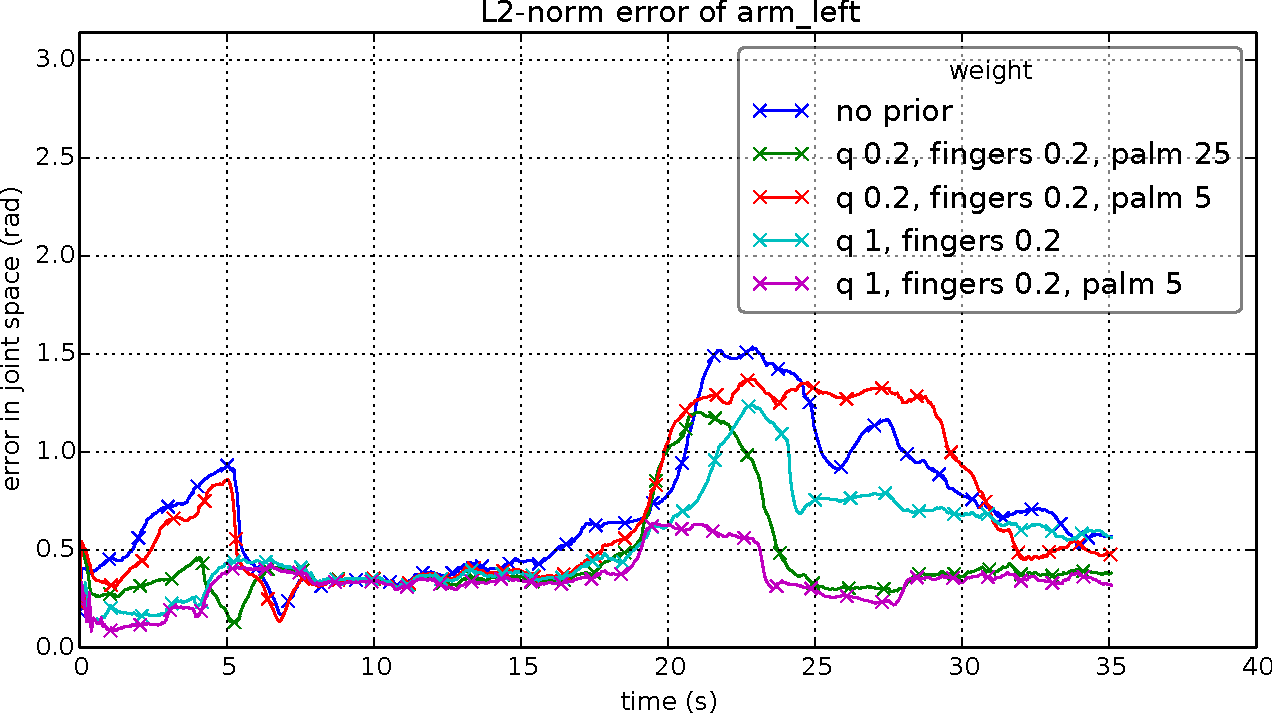
\includegraphics[width=0.5\textwidth]{images/eval_prior/inidv_weights/stereo_arm_joint_error.pdf} \label{fig:indiv_joint_error_arm}}

\caption{Joint space error for individual weighting}
\label{fig:indiv_joint_error}
\end{figure}

Again, the arm joints directly influence the pose error of the hand as seen in \cref{fig:indiv_pose_error}. \Cref{fig:indiv_hand_pos_error} shows that the hand position mostly benefits from using some weight $>1$ on the palm joints whereas weighting the remaining joints does not contribute to driving the solution towards the reported hand position. For the hand orientation error in \cref{fig:indiv_hand_ori_error}, the error is usually reduced if the weights on the palm joints are increased (e.g. $1$ to $5$, or $5$ to $25$) and remaining joints keep their weights. We can also see that using small weights ($q=0.2$) for all joints but the palm actually results in a estimated position closer to the reported position than what is achieved by larger weights ($q=1$).

\begin{figure}
\centering
\subfloat[]{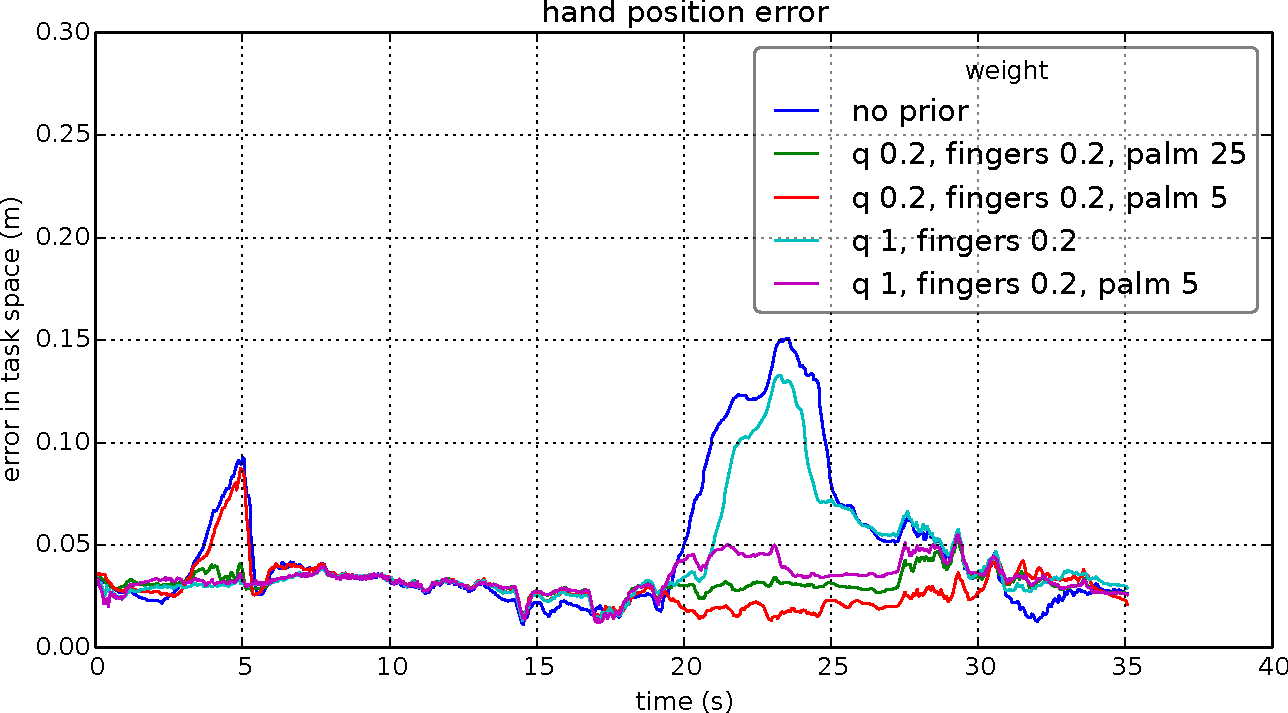
\includegraphics[width=0.5\textwidth]{images/eval_prior/inidv_weights/stereo_hand_pos_error.pdf} \label{fig:indiv_hand_pos_error}}
%
\subfloat[]{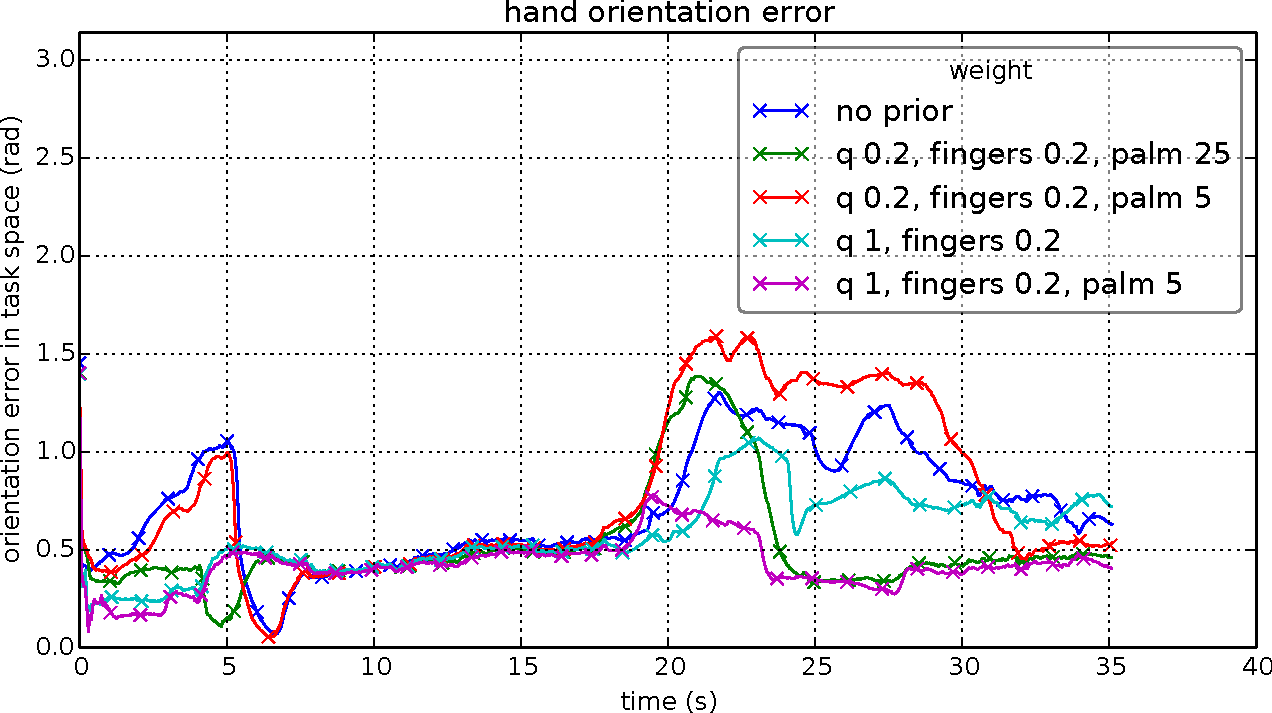
\includegraphics[width=0.5\textwidth]{images/eval_prior/inidv_weights/stereo_hand_ori_error.pdf} \label{fig:indiv_hand_ori_error}}

\caption{Task space error for individual weighting}
\label{fig:indiv_pose_error}
\end{figure}

\subsubsection{Object Position}

Most of the time, the pose of the object (bottle) is mainly affected by the optimization. Only when there is interaction between the manipulator and the object, it gets indirectly dependant on the joint values and hence the prior weight. The object's pose is initialise close to the true observed state and is expected to not move until the end of the reaching phase. \Cref{fig:bottle_movement} compares the object's distance to the image origin for stereo and xtion datasets and gives an indication about its movement. The bottle in the stereo data (\cref{fig:bottle_movement_stereo}) stays, as expected, close to its initial position until the end of the reaching phase. In contrast, the bottle in the Xtion dataset (\cref{fig:bottle_movement_xtion}) already moves at the beginning to its final pose.

\begin{figure}
\centering
\subfloat[stereo]{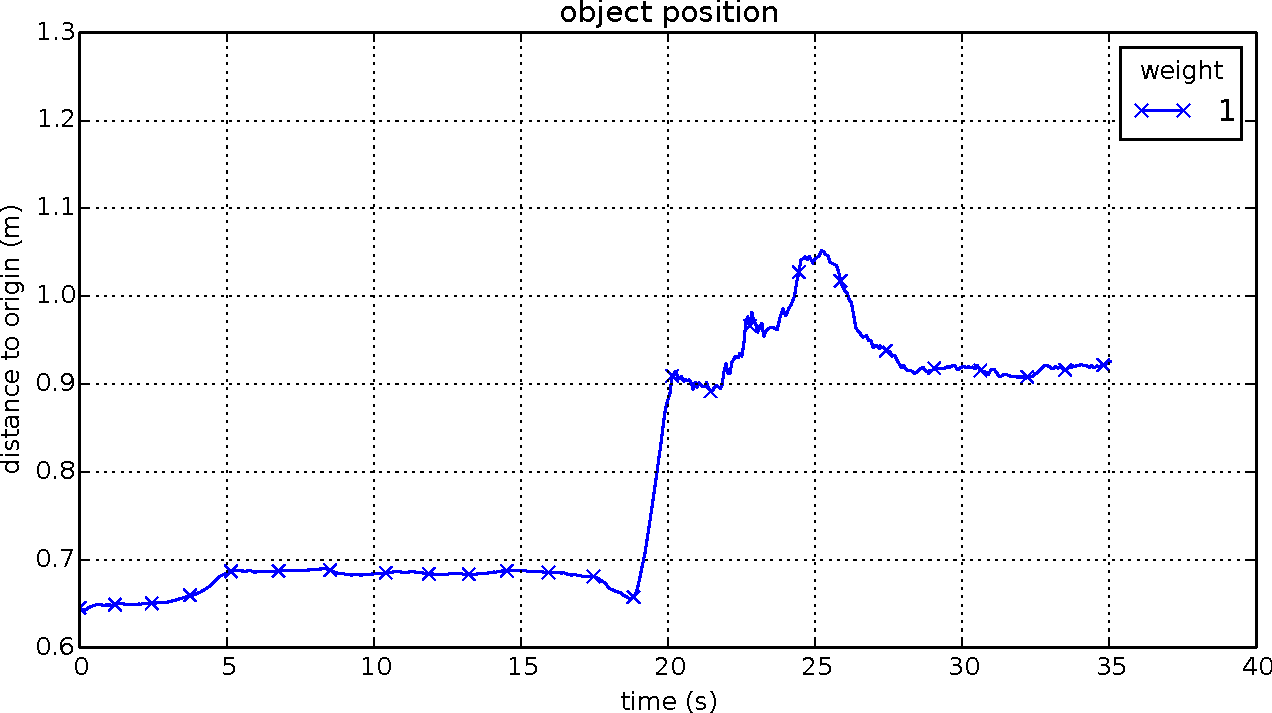
\includegraphics[width=0.5\textwidth]{images/eval_prior/stereo_obj_pos.pdf} \label{fig:bottle_movement_stereo}}
\subfloat[xtion]{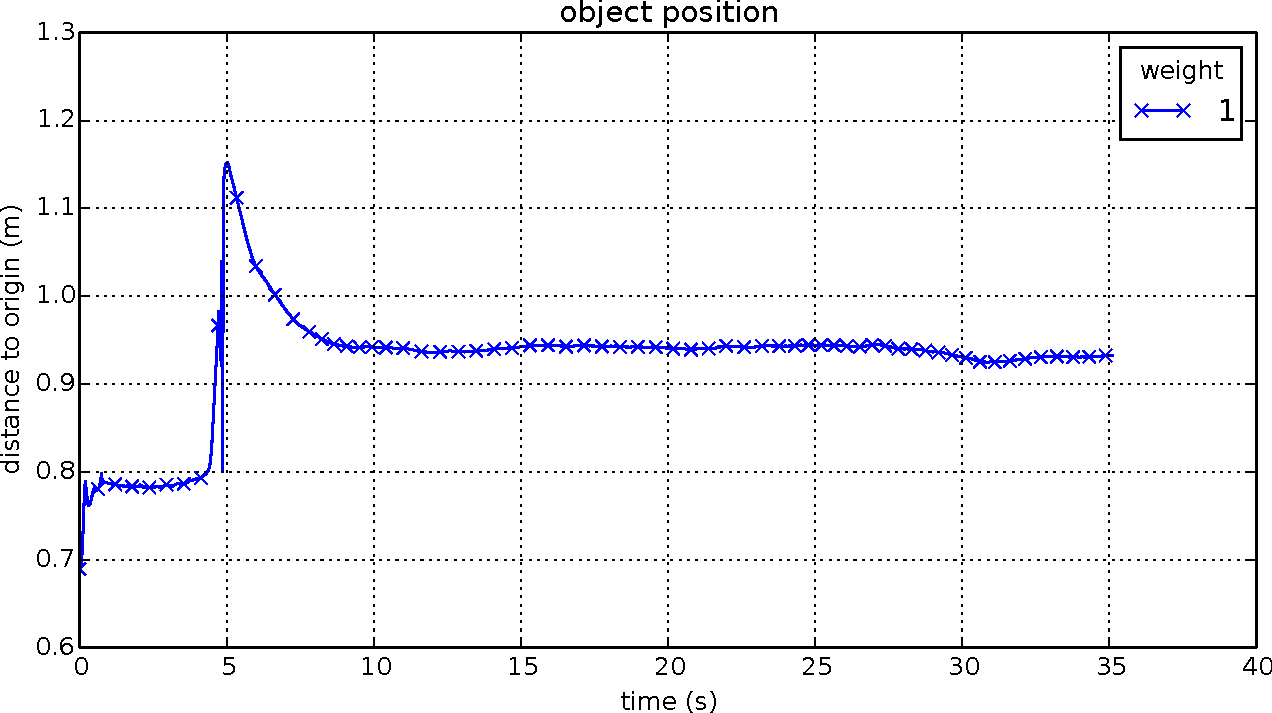
\includegraphics[width=0.5\textwidth]{images/eval_prior/xtion_obj_pos.pdf} \label{fig:bottle_movement_xtion}}
\caption{Movement of bottle during robot arm movement}
\label{fig:bottle_movement}
\end{figure}

A snapshot of the perceived point cloud is depicted in \cref{fig:bottle_point_cloud} for a state at the beginning of the experiment for both depth sources. A comparison of these sources show that: 1) the stereo depth source contains data with larger depth, and 2) the stereo depth source also contains more points of the object than the structured light sensor. It must be noted that the structured light sensor is mounted above the stereo sensor pointing into the same region of interest. It thus perceives the scene at a steeper angle.

\begin{figure}
\centering
\subfloat[stereo point cloud]{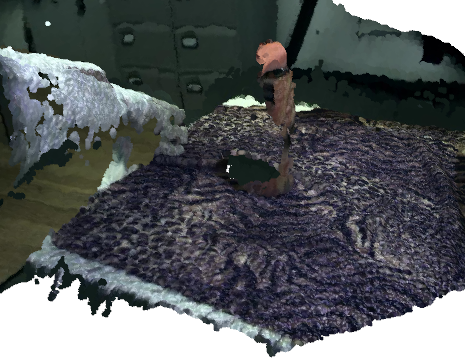
\includegraphics[width=0.4\textwidth]{images/eval_prior/stereo_bottle.png} }
\hspace{1cm}
\subfloat[xtion point cloud]{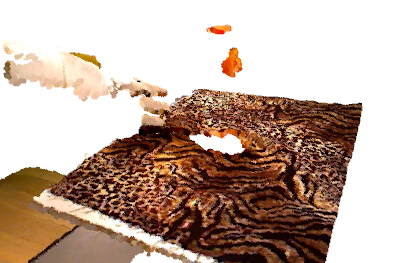
\includegraphics[width=0.4\textwidth]{images/eval_prior/xtion_bottle.png} }
\caption{Table and bottle in stereo and xtion point cloud}
\label{fig:bottle_point_cloud}
\end{figure}

\subsection{Interpretation}

With the signed distance as the only objective function, the optimization is driven away from the reported state, with which it is initialized, whenever nearby but unrelated depth data is assigned to the robot model. Hence we conclude that \cref{hyp:distracting_readings} is true. By augmenting the objective function with an objective related to the reported state as the reference, these issues can be faced.

Across all weighting schemes and depth sources, we can see that weighting in respect to the deviation from the reported pose: (1) reduces the deviation of finger joint positions over the whole sequence of the trials by already choosing a small prior weight, (2) contributes most in movement phases that follow states where the manipulator is in contact with the scene (table, object). The application of individual weighting of joint deviations showed that by selecting specific joints, the task space error can be reduced while keeping the flexibility of preferring other objectives for remaining parts of the robot model. For both assessed weighting schemes, it turned out that weights need to be chosen carefully to prevent overshooting on the reported state and hence the oscillation of estimate. Neglecting the issue of oscillating around the optimum, \cref{hyp:prior_information} is also considered as verified.

The assessed prior information is by design only applicable to the robot model; the tracked object remains to be driven by the signed distance function and hence relies on relevant depth data assigned to the object model. We saw that this is an issue for observing from an low angle to the object's principal axes.


\section{True Hand Pose Error}
\label{sec:hand_pose_error}

An experiment is conducted that contains depth data measurement from the manipulator alone, without distracting depth readings nearby. As in a previous experiment, forward kinematics on the reported and estimated joint configuration will be used to obtain the pose of the manipulator in task space. Additionally, the Vicon system introduced earlier provides ground truth data of the hand palm pose.


\subsection{Hypotheses}

The experiment has been designed to (1) apply the tracking of the manipulator in a scene without distractions, and (2) to compare the reported and estimated robot configuration with the as ground truth defined poses reported by the Vicon tracking system.

Without distracting sensor readings, we expect that the use of the joint position prior will not have a strong impact on the deviation from the reported robot configuration. If the manipulator is fully observed in the depth data, tracking the manipulator should result in a hand pose close to the true hand pose which itself should coincide with the reported hand pose.

\begin{hypothesis}(No effect of joint position prior)\\
There will be no significant effect of applying joint position prior on observations containing solely the manipulator.
\label{hyp:no_prior_effect}
\end{hypothesis}

\begin{hypothesis}(Matching hand pose)\\
Reported and estimated left hand pose agree with the true measured hand pose.
\label{hyp:matching_hand_pose}
\end{hypothesis}


\subsection{Setup}

The robot is placed in nominal position and its manipulator is moving from this state into the field of view of the camera (\cref{fig:vicon_free_movement}). To observe the manipulator and its fingers from different perspectives, the hand and the fingers are actuated by a certain degree. The data set is therefore divided into two parts: \textit{arm movement}, where mainly the shoulder and the forearm joints are commanded, and \textit{finger movement} where all fingers are actuated at the same time. During the complete experiment, Vicon markers are attached to the pelvis and backside of the palm to track the orientation of both robot frames.

The \textit{arm movement} sequence contains three phases (\cref{tab:vic_arm_movement_phases}) of which 3 final states are depicted in \cref{fig:arm_movement_states}. The \textit{finger movement} sequence contains 7 phases in total (\cref{tab:vic_finger_movement_phases}) of which 6 states are depicted in \cref{fig:finger_movement_states}. Both sequences show that due to self-occlusion, the manipulator cannot be fully observed in a single time instance. In states where the palm is facing the robot or down, the Vicon marker can be observed in the point cloud data.

%It can be noticed that the reported state of the finger joint positions does not resemble the true articulation.

\begin{figure}
\captionsetup{width=0.4\textwidth}
\centering
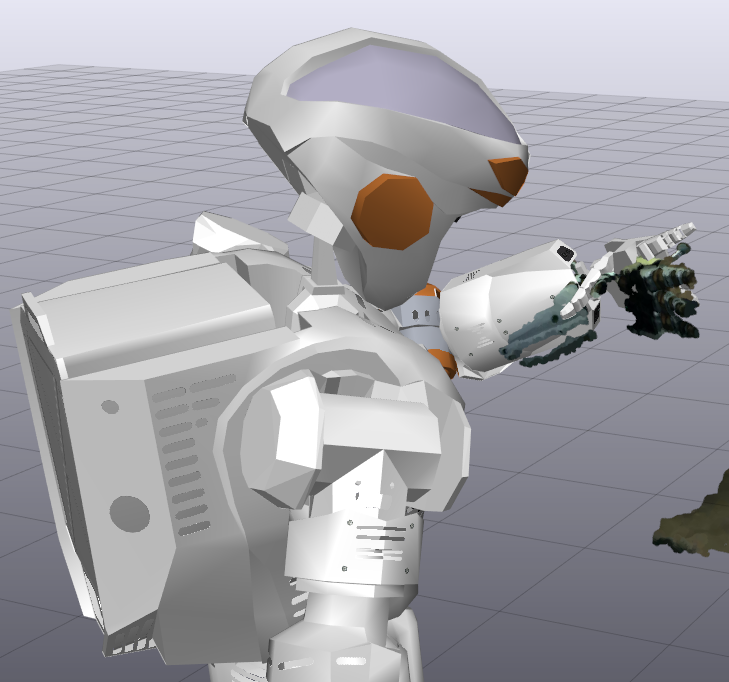
\includegraphics[width=0.4\textwidth]{images/eval_vicon/sequence/setting.png}
\caption{Setup in which a robot is observing its own manipulator.}
\label{fig:vicon_free_movement}
\end{figure}

\begin{table}
\centering
\begin{tabular}{|c|l|l|}
\hline
 & \emph{time (s)} & \emph{movement description} \\
\hline
1 & 0$\dots$50 & no movement, hand in lower camera view \\
\hline
2 & 50$\dots$54 & arm movement up \\
\hline
3 & 85$\dots$90 & hand palm turning up (forearm joint) \\
\hline
4 & 125$\dots$130 & hand palm turning down (forearm joint) \\
\hline
\end{tabular}
\caption{Phases of arm movement}
\label{tab:vic_arm_movement_phases}
\end{table}

\begin{figure}
\centering
\begin{tabular}{c:c:c}
\textit{t=55} & \textit{t=91} & \textit{t=132} \\
(facing towards robot) & (facing up) & (facing down)\\
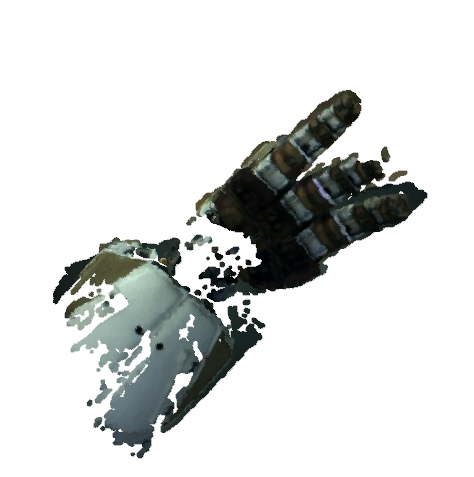
\includegraphics[width=0.3\textwidth]{images/eval_vicon/sequence/arm_movement/obs_55.png} & 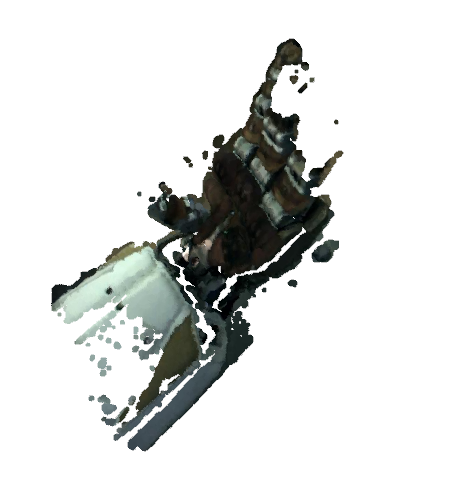
\includegraphics[width=0.3\textwidth]{images/eval_vicon/sequence/arm_movement/obs_91.png} & 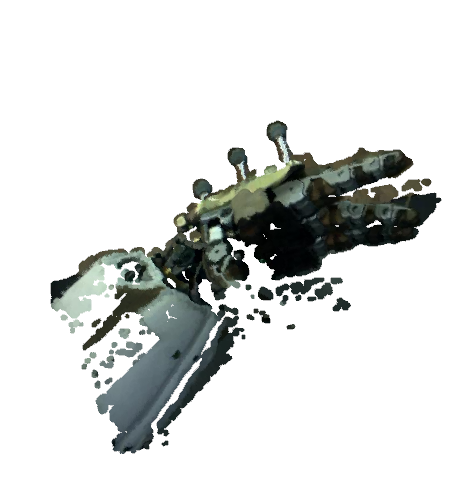
\includegraphics[width=0.3\textwidth]{images/eval_vicon/sequence/arm_movement/obs_132.png} \\
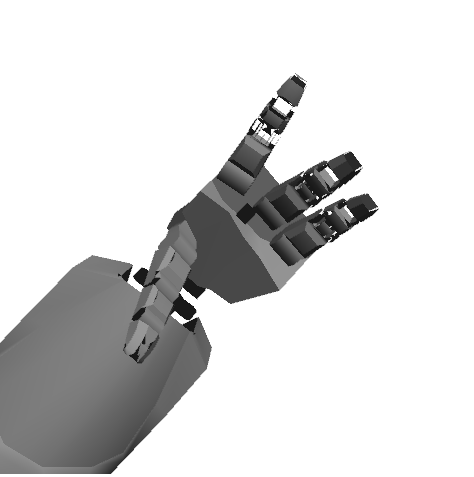
\includegraphics[width=0.3\textwidth]{images/eval_vicon/sequence/arm_movement/rep_55.png} & 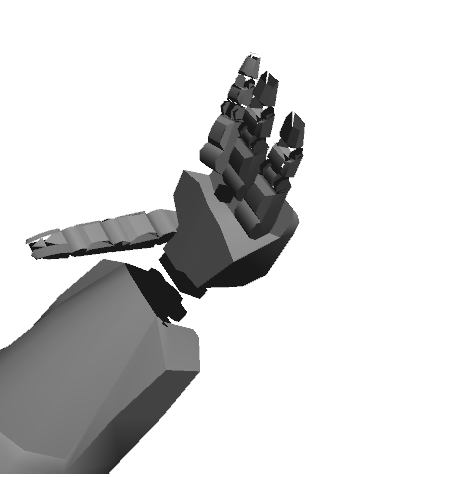
\includegraphics[width=0.3\textwidth]{images/eval_vicon/sequence/arm_movement/rep_91.png} & 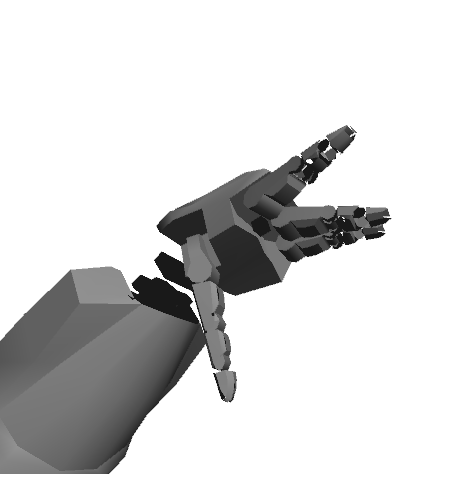
\includegraphics[width=0.3\textwidth]{images/eval_vicon/sequence/arm_movement/rep_132.png} \\
\end{tabular}
\caption[Arm movement sequence]{Arm movement: Sequence of states in which the manipulator is observed from different viewing angles. \textit{Upper row:} point cloud observation, \textit{Lower row:} reported state.}
\label{fig:arm_movement_states}
\end{figure}


\begin{table}
\centering
\begin{tabular}{|c|l|l|}
\hline
 & \emph{time (s)} & \emph{movement description} \\
\hline
1 & 0$\dots$30 & no movement, palm facing towards camera \\
\hline
2 & 30$\dots$33 & fingers closing 25\% \\
\hline
3 & 56$\dots$59 & fingers closing 50\% \\
\hline
4 & 72$\dots$75 & fingers opening \\
\hline
5 & 100$\dots$104 & hand palm turning up (forearm joint) \\
\hline
6 & 127$\dots$130 & fingers closing 25\% \\
\hline
7 & 147$\dots$150 & fingers closing 50\% \\
\hline
8 & 156$\dots$159 & fingers opening \\
\hline
\end{tabular}
\caption{Phases of finger movement}
\label{tab:vic_finger_movement_phases}
\end{table}

\begin{figure}
\centering
\begin{tabular}{c:c:c}
\hline
\textit{t=19} & \textit{t=33} & \textit{t=61}\\
(opened) & (closed $\sim 25\%$) & (closed $\sim 50\%$)\\
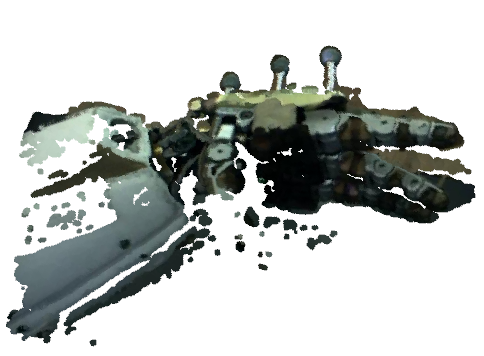
\includegraphics[width=0.3\textwidth]{images/eval_vicon/sequence/finger_movement/obs_0.png} & 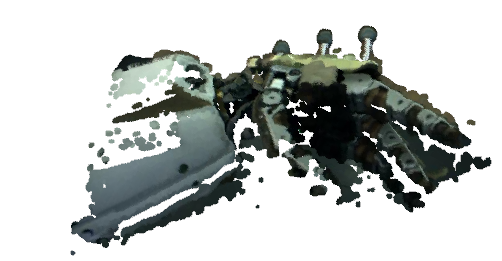
\includegraphics[width=0.3\textwidth]{images/eval_vicon/sequence/finger_movement/obs_33.png} & 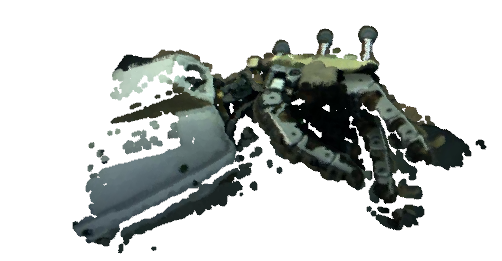
\includegraphics[width=0.3\textwidth]{images/eval_vicon/sequence/finger_movement/obs_61.png} \\
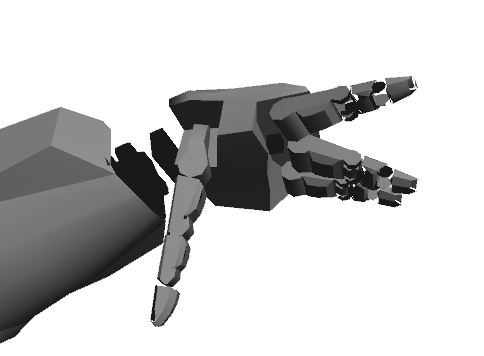
\includegraphics[width=0.3\textwidth]{images/eval_vicon/sequence/finger_movement/rep_0.png} & 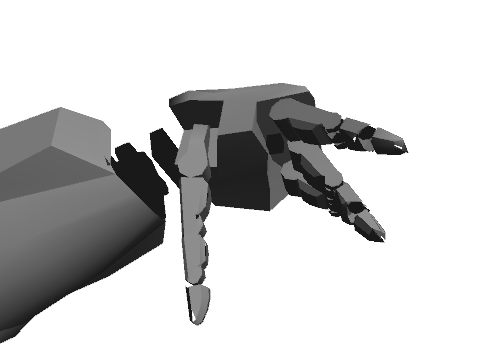
\includegraphics[width=0.3\textwidth]{images/eval_vicon/sequence/finger_movement/rep_33.png} & 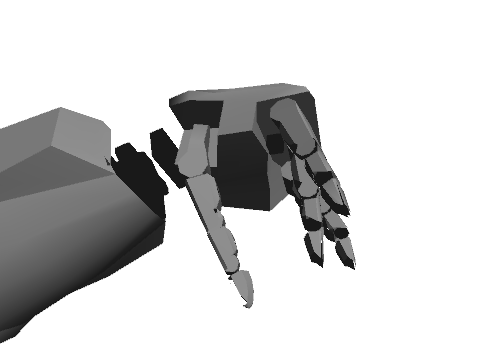
\includegraphics[width=0.3\textwidth]{images/eval_vicon/sequence/finger_movement/rep_61.png} \\
\hline
\textit{t=105} & \textit{t=133} & \textit{t=152}\\
(opened) & (closed $\sim 25\%$) & (closed $\sim 50\%$)\\
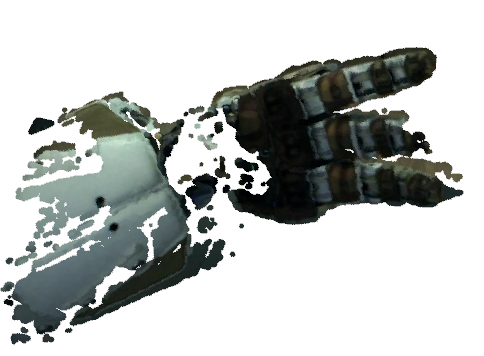
\includegraphics[width=0.3\textwidth]{images/eval_vicon/sequence/finger_movement/obs_105.png} & 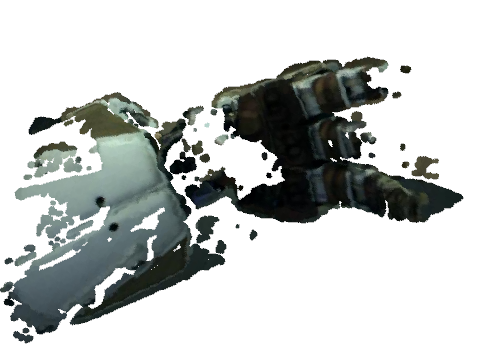
\includegraphics[width=0.3\textwidth]{images/eval_vicon/sequence/finger_movement/obs_133.png} & 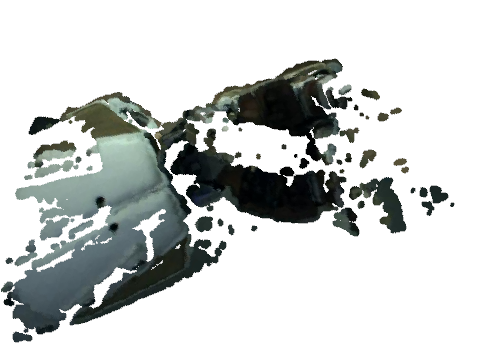
\includegraphics[width=0.3\textwidth]{images/eval_vicon/sequence/finger_movement/obs_152.png} \\
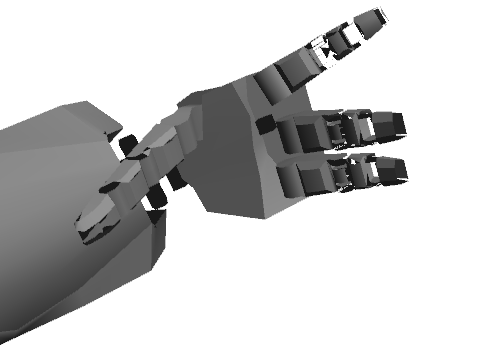
\includegraphics[width=0.3\textwidth]{images/eval_vicon/sequence/finger_movement/rep_105.png} & 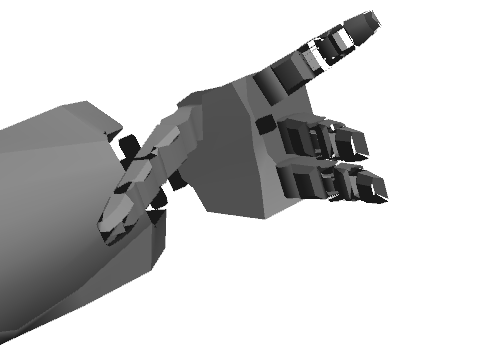
\includegraphics[width=0.3\textwidth]{images/eval_vicon/sequence/finger_movement/rep_133.png} & 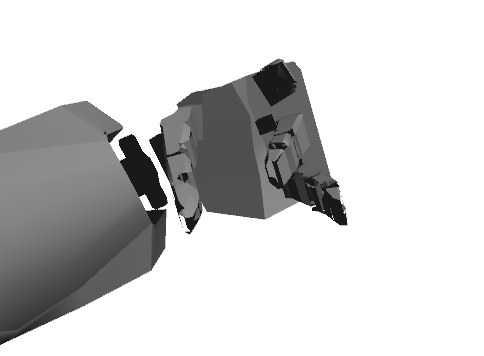
\includegraphics[width=0.3\textwidth]{images/eval_vicon/sequence/finger_movement/rep_152.png} \\
\end{tabular}
\caption[Finger movement sequence]{Finger movement: Sequence of states in which the fingers are close to certain degree (open, closed $\sim 25\%$, closed $\sim 50\%$). \textit{Upper sequence:} Hand palm facing down, \textit{Lower sequence:} Hand palm facing towards robot. In each sequence: \textit{Upper row:} point cloud observation, \textit{Lower row:} reported state.}
\label{fig:finger_movement_states}
\end{figure}


\subsection{Results}

The shown errors are the L2 norm of the joint and task space errors as defined in \cref{sec:prior_results}. The common weighting scheme \emph{Weighted L2 norm of joint position deviation} (objective function \cref{eqn:objf_weightedL2}) is applied for the joint position prior when comparing different weights. Time and duration is given in seconds.

\subsubsection{Joint Space Error}

The joint space error for both sequences is shown separately for finger and arm joints in \cref{fig:am_joint_error,fig:fm_joint_error}. It can be noticed that increasing prior weights reduces the joint position deviation also in the case of less distracting observations. In contrast, the effect is not as significant as it is for observations with distractions due to close solutions after proper initialisation.

\begin{figure}
\centering
\subfloat[]{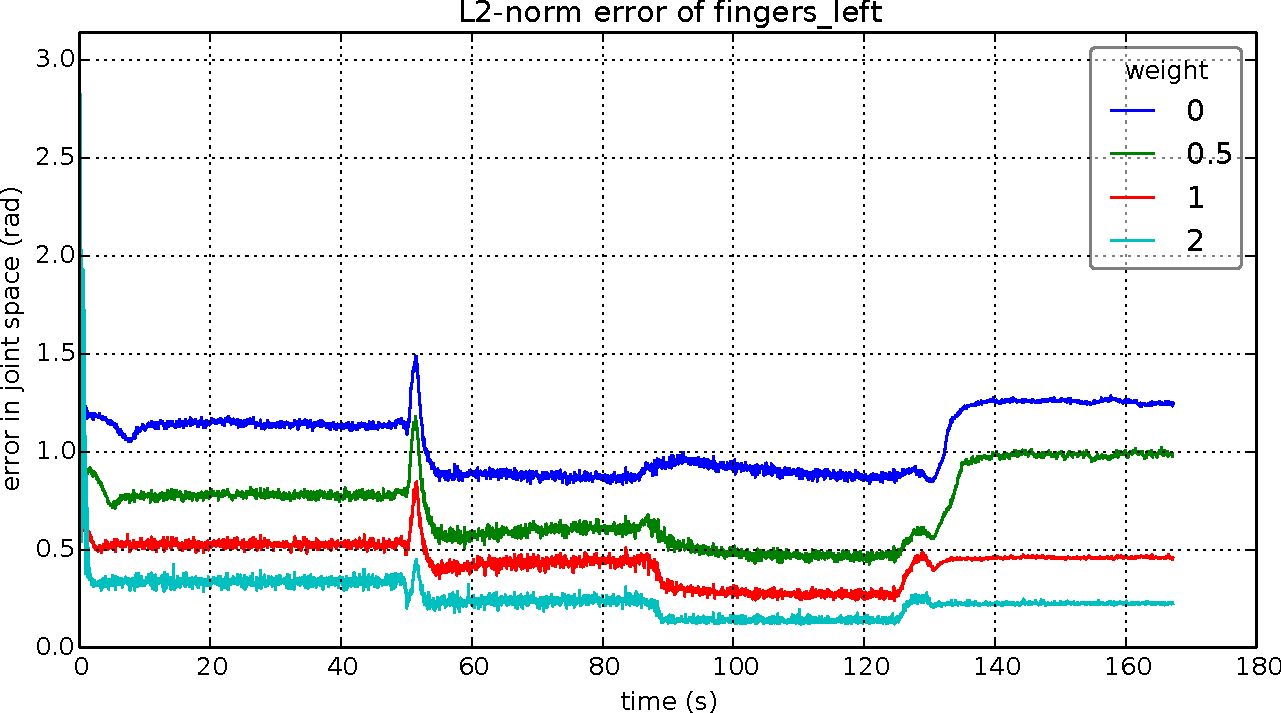
\includegraphics[width=0.5\textwidth]{images/eval_vicon/val_arm_joint_error_fingers.pdf} }
\subfloat[]{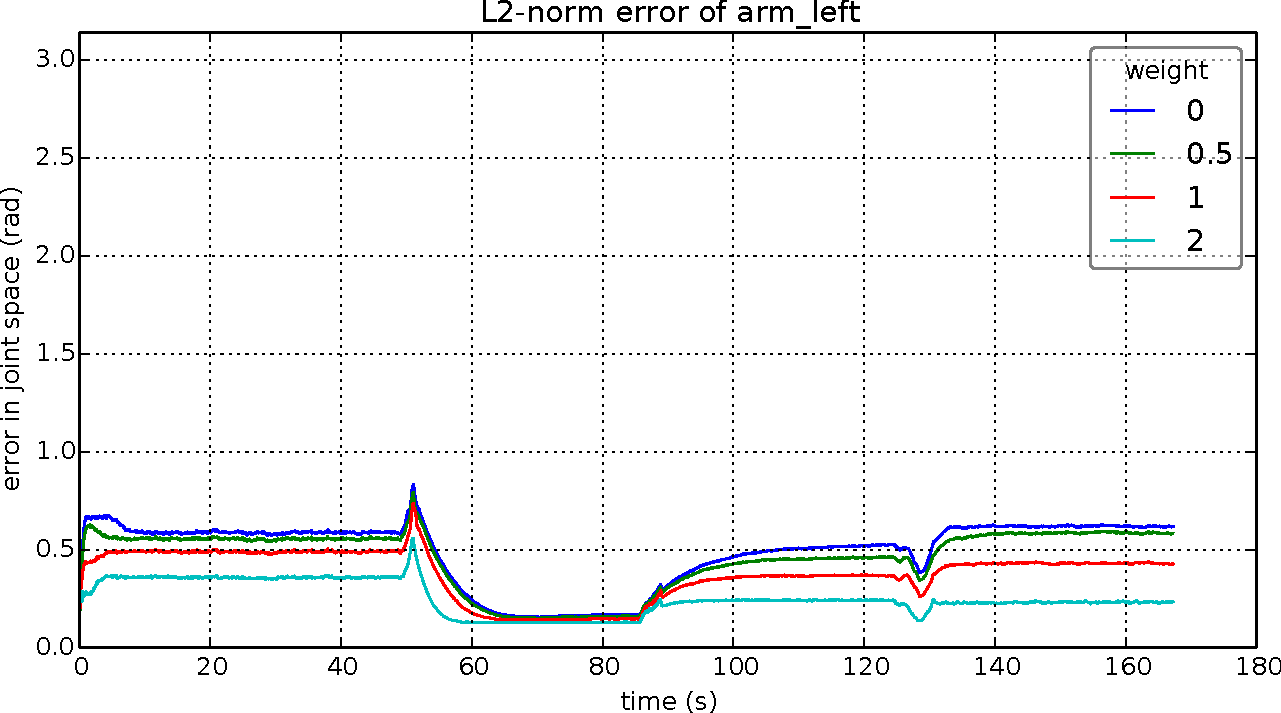
\includegraphics[width=0.5\textwidth]{images/eval_vicon/val_arm_joint_error_arm.pdf} }
\caption{Arm movement, joint space error}
\label{fig:am_joint_error}
\end{figure}

\begin{figure}
\centering
\subfloat[]{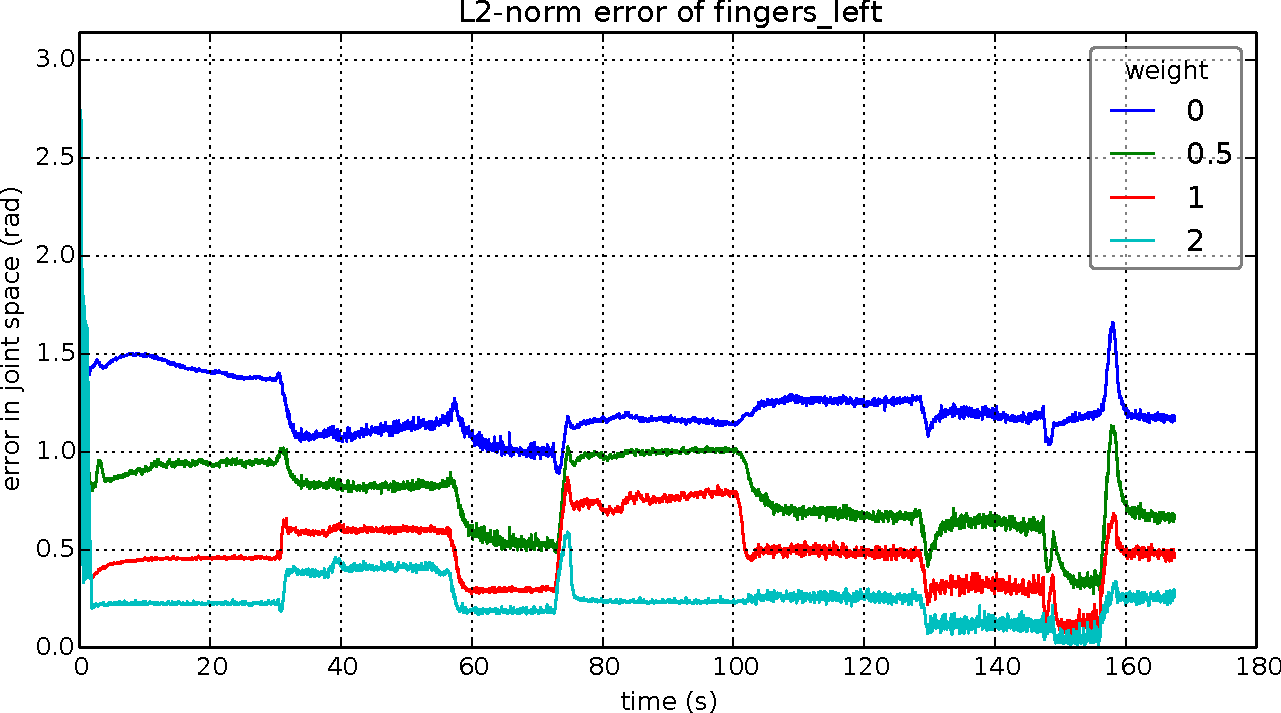
\includegraphics[width=0.5\textwidth]{images/eval_vicon/val_finger_joint_error_fingers.pdf} }
\subfloat[]{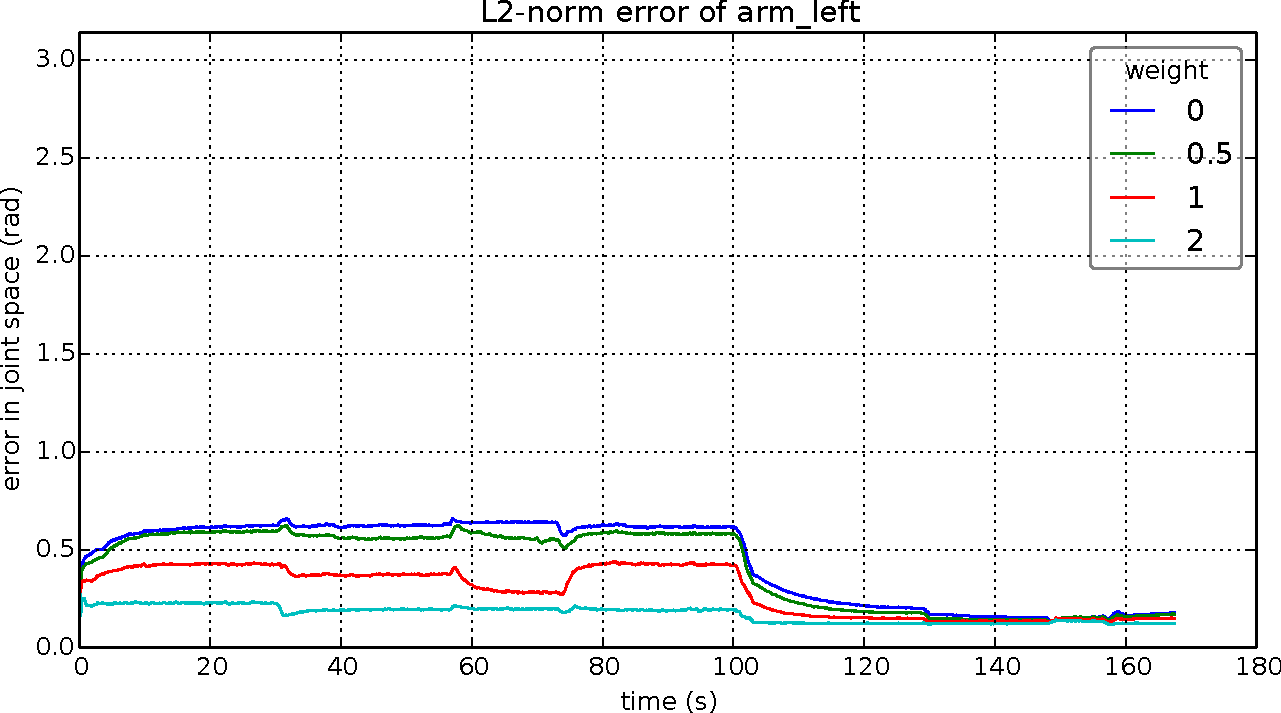
\includegraphics[width=0.5\textwidth]{images/eval_vicon/val_finger_joint_error_arm.pdf} }
\caption{Finger movement, joint space error}
\label{fig:fm_joint_error}
\end{figure}

In states where the palm is facing towards the camera and large continuous hand parts can be observed, the tracked configuration is already so close to the reported configuration, that an additional joint position prior has no effect. This is the case after phase 2 for the \textit{arm movement} data set ($55\leq t \leq84$) and phase 5 for the \textit{finger movement} data set ($t \geq 105$).


\subsubsection{Task Space Error}

For the evaluation of the task space error, we compare the reported and the estimated hand pose with the hand pose from the Vicon tracking system. The shown errors are the L2 norm of the 3D pose and 3D rotation difference from Vicon pose to reported and estimated pose.

The error plots in \cref{fig:vic_error_arm_movement,fig:vic_error_finger_movement} compare the effect of prior weighting on the estimated configurations against the reported configuration (which is not effected by the prior). Comparison plots for the task space error on the reported and on the estimated pose without prior are shown separately for a clearer distinction.

\begin{figure}
\centering
\subfloat[position error]{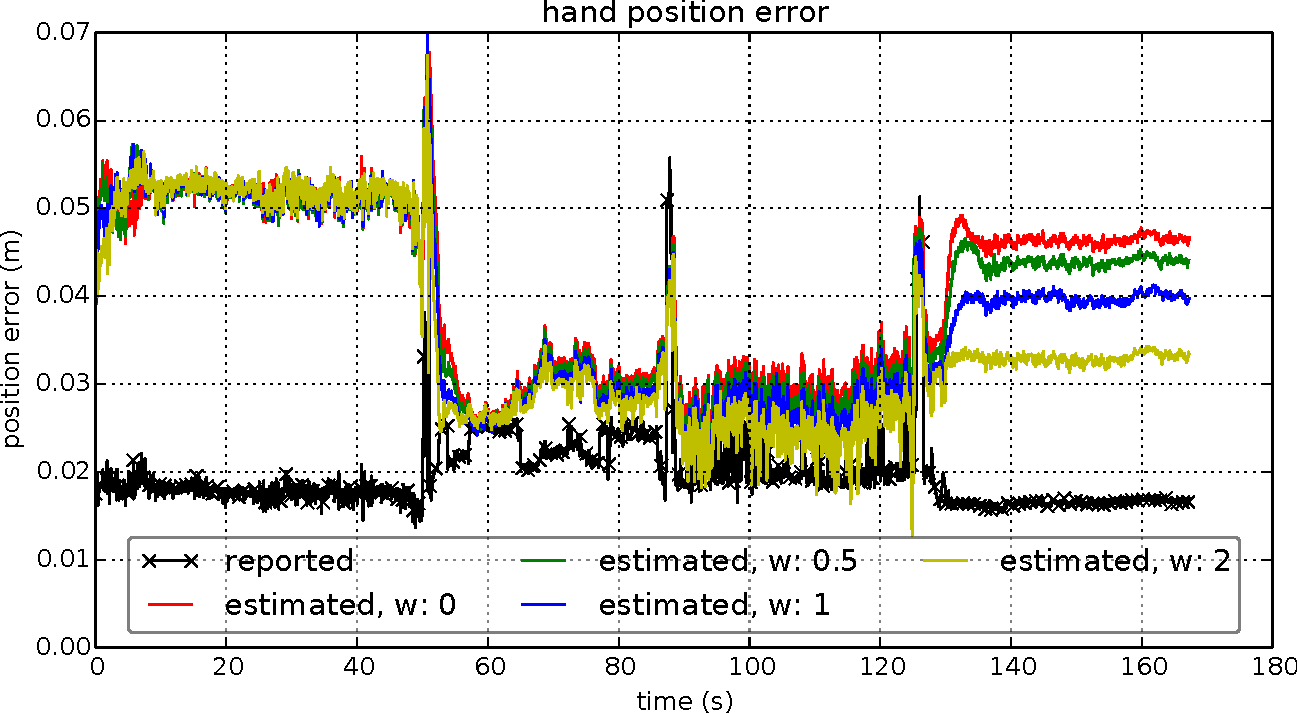
\includegraphics[width=0.5\textwidth]{images/eval_vicon/val_arm_pos_error.pdf} }
\subfloat[orientation error]{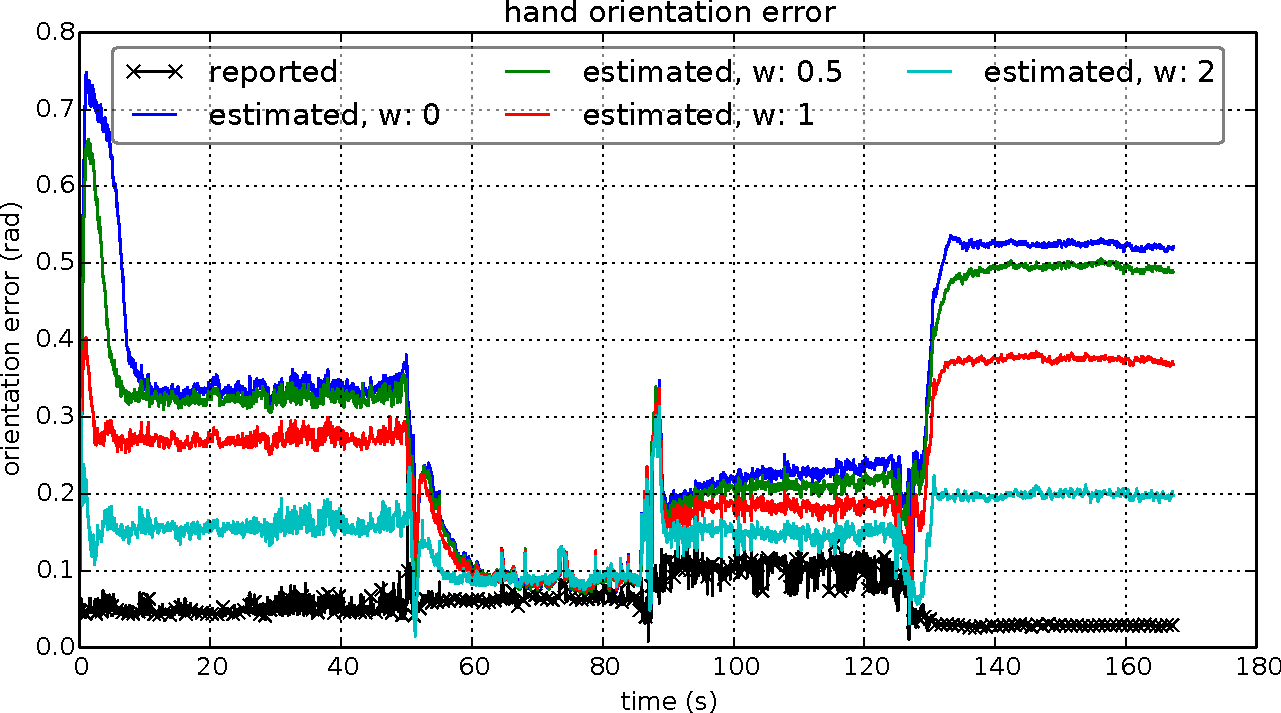
\includegraphics[width=0.5\textwidth]{images/eval_vicon/val_arm_ori_error.pdf} }

\subfloat[position error (no prior)]{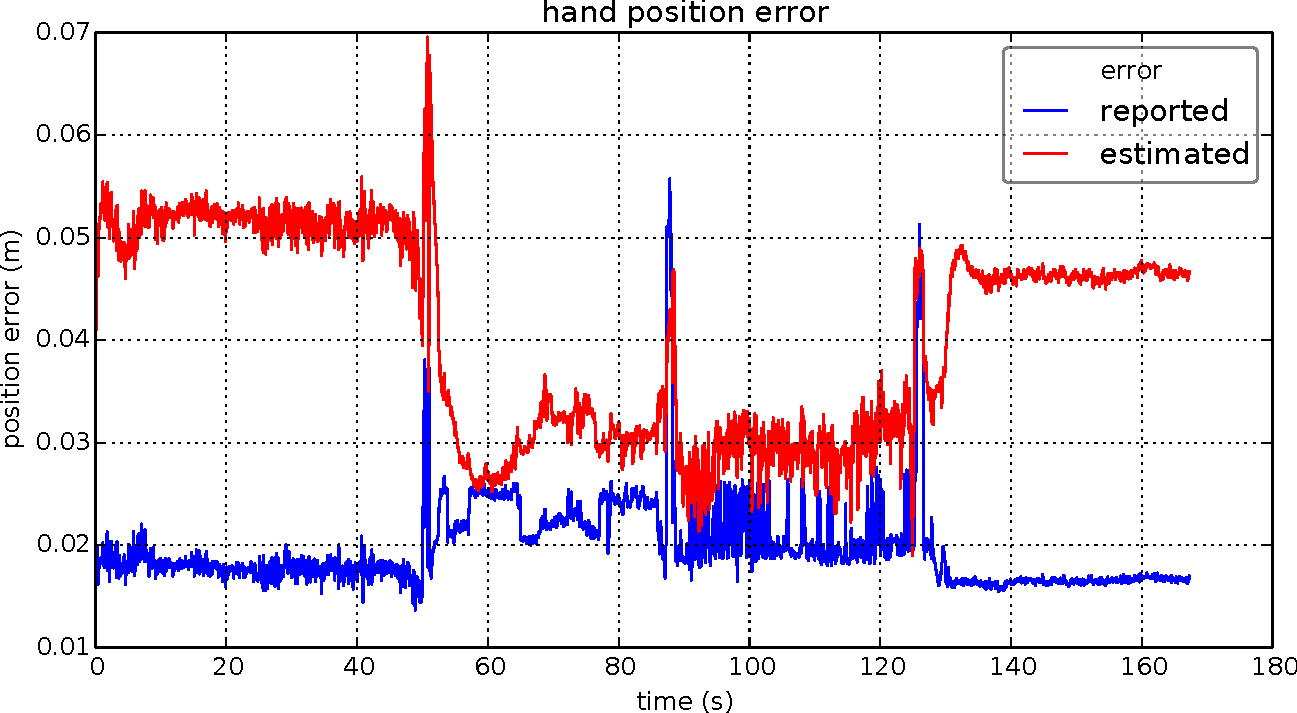
\includegraphics[width=0.5\textwidth]{images/eval_vicon/val_arm_pos_error_nop.pdf} }
\subfloat[orientation error (no prior)]{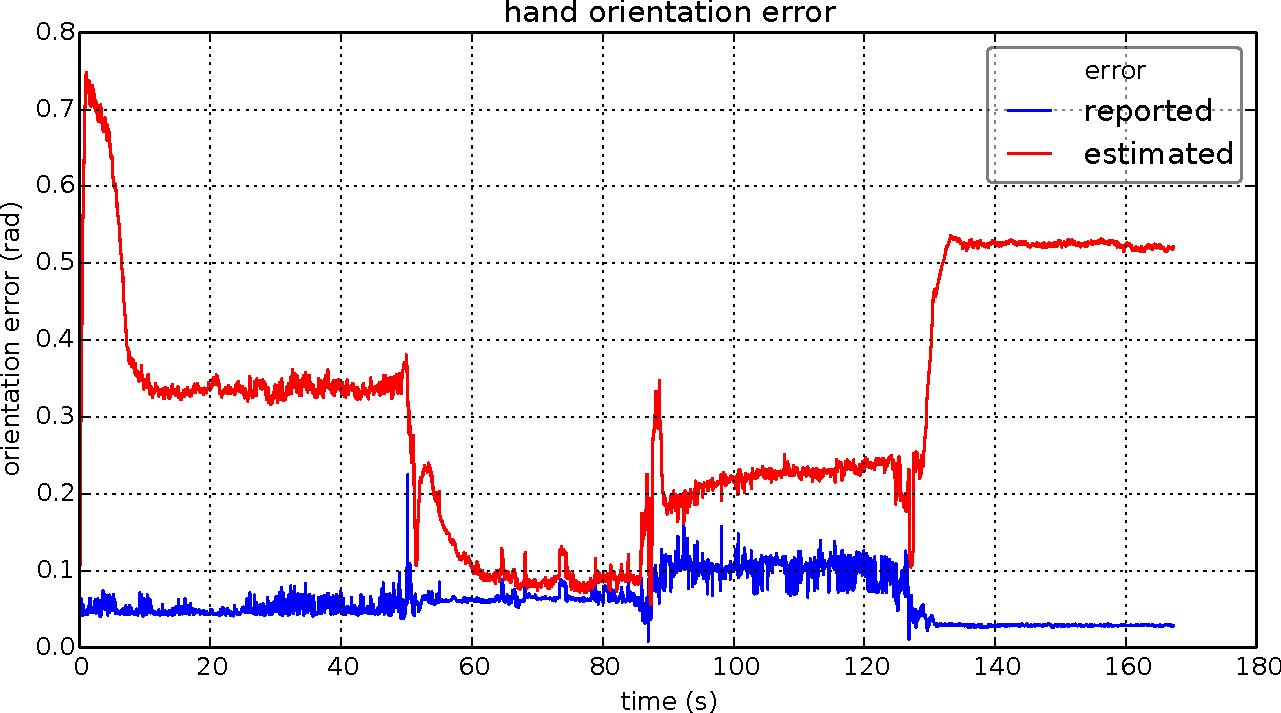
\includegraphics[width=0.5\textwidth]{images/eval_vicon/val_arm_ori_error_nop.pdf} }

\caption[Arm movement, hand pose error]{Arm movement, Hand pose error of reported and estimated robot state compared to Vicon hand marker pose.}
\label{fig:vic_error_arm_movement}
\end{figure}

The following general statements can be made: (1) neither the reported nor the estimated hand poses agree with the Vicon hand pose, (2) the reported hand pose is closer to the Vicon hand pose than the estimated hand pose for most of the duration.

From both data sets it can be noticed that the estimated pose is closer to the Vicon pose in the same states where the joint deviation from the reported configuration is small. Especially the orientation error drops significantly in these states where large portions of the palm are observable (\textit{arm movement}: $55\leq t \leq84$, \textit{finger movement}: $t \geq 105$). In contrast, the error increases when the manipulator is observed from the side, e.g. when fingers are occluding each other.

\begin{figure}
\centering
\subfloat[position error]{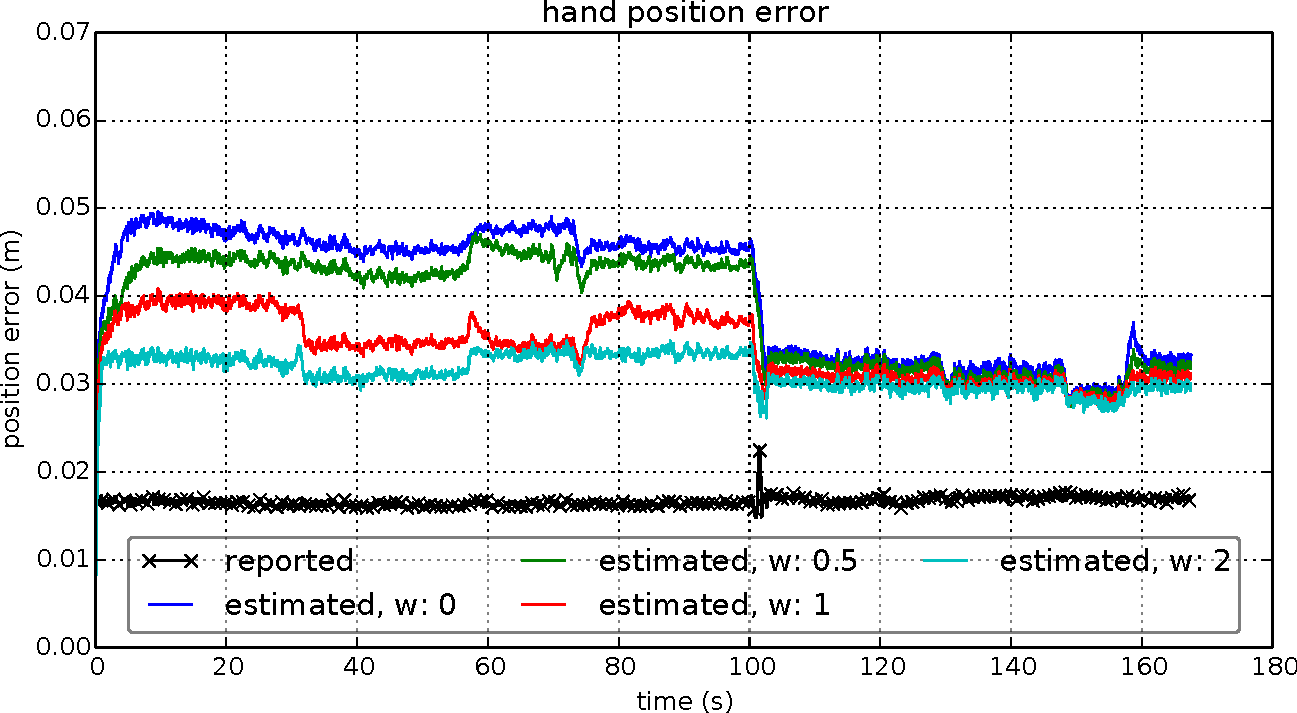
\includegraphics[width=0.5\textwidth]{images/eval_vicon/val_finger_pos_error.pdf} }
\subfloat[orientation error]{\includegraphics[width=0.5\textwidth]{images/eval_vicon/val_finger_ori_error.pdf} }

\subfloat[position error (no prior)]{\includegraphics[width=0.5\textwidth]{images/eval_vicon/val_finger_pos_error_nop.pdf} }
\subfloat[orientation error (no prior)]{\includegraphics[width=0.5\textwidth]{images/eval_vicon/val_finger_ori_error_nop.pdf} }

\caption[Finger movement, hand pose error]{Finger movement, Hand pose error of reported and estimated robot state compared to Vicon hand marker pose.}
\label{fig:vic_error_finger_movement}
\end{figure}


\subsection{Interpretation}

Tracking with manipulator only observed data showed, that there is still an effect of using prior information. However, this effect is not as significant as in distracting scenes and it is minimal in states where large portions of the manipulator can be observed in a single time instance. The performance of the tracking and hence the effect of prior information is view dependent. Prior information is still useful for inconclusive observations, e.g. self-occlusion. Despite this, \cref{hyp:no_prior_effect} is considered as true.

The observation of the Vicon marker in the depth data of the manipulator, e.g. when the hand palm is facing down, is not examined in this evaluation. These markers are required to obtain the ground truth data but they certainly provide  readings that could distract the optimization.

An interesting result from this evaluation is that neither the reported nor the estimated hand pose agree with the Vicon hand pose. The measured discrepancy of reported position and Vicon marker position is at least \SI{1.5}{\cm}. Using strong prior in such scenario thus can only provide an optimal solution to some extent, e.g. as long as the reported configuration is closer to the true configuration than the estimate. \Cref{hyp:matching_hand_pose} is considered as not verified and needs further investigation.


\section{Joint Calibration}

The data set collected in the previous experiment in \cref{sec:hand_pose_error} will be used to investigate the issue of mismatching hand poses of the reported and estimated state from the Vicon hand pose that is considered as ground truth.

\subsection{Hypothesis}

Under the assumption that the tracking obtains the true robot configuration, that is the estimated hand pose agrees with the Vicon hand pose, the joint position discrepancy (1) from reported configuration to configuration at Vicon pose, and (2) from reported configuration to estimated configuration, should be similar.

\begin{hypothesis}(Matching joint offset)\\
The joint position offset from reported configuration to both Vicon configuration and estimated configuration are similar.
\label{hyp:matching_joint_offset}
\end{hypothesis}

\subsection{Results}

The individual arm joint position offsets for the arm movement and finger movement data sets (\cref{fig:estimated_offsets}) show that the discrepancy of estimated to reported joints position is mostly not constant overt time. Considering that the hand is directly connected to the forearm by two joints (\texttt{leftWristRoll/Pitch}), it is interesting to notice that \texttt{leftWristPitch} does not have a discrepancy to the reported joint position value.

\Cref{tab:avg_offsets_comparison} summarizes the offsets for the estimated (\textit{dart}, averaged over time) and reported (\textit{vicon}, optimized on pose) joint position offsets. As the manipulator tracking considers the kinematic chain from image centre to palm and the Vicon marker pose gives the final transformation for the kinematic chain from pelvis to palm, the arm joints are the common joints whose offsets are considered for comparison.
The correlation between the averaged \textit{dart} offsets and \textit{vicon} offsets are given as $0.3366$ for the arm data set and $0.1054$ for the finger data set.

\begin{figure}
\centering
\subfloat[Arm movement]{\includegraphics[width=0.5\textwidth]{images/offset/dart_arm_offset.pdf} }
\subfloat[Finger movement]{\includegraphics[width=0.5\textwidth]{images/offset/dart_finger_offset.pdf} }

\caption[Estimated offsets]{Estimated offsets of reported joint configuration to estimated configuration}
\label{fig:estimated_offsets}
\end{figure}


\begin{table}
\centering
% table with aligned decimal points
\begin{tabular}{|l||S[table-format=2.5]|S[table-format=2.5]||S[table-format=2.5]|S[table-format=2.5]||>{\columncolor[gray]{0.9}}S[table-format=2.8]|}
\hline
 & \multicolumn{5}{c|}{joint positions offsets} \\
\hline
 & \multicolumn{2}{c||}{arm dataset} & \multicolumn{2}{c||}{finger dataset} &  \multicolumn{1}{c|}{complete} \\
\hline
\multicolumn{1}{|c||}{\textit{joint name}} & \textit{dart} & \textit{vicon} & \textit{dart} & \textit{vicon} & \multicolumn{1}{c|}{\textit{vicon}} \\
\hline
\hline
\texttt{torsoYaw} &  & 0.00059 &  & -0.00118 & 0.01319969 \\
\hline
\texttt{torsoPitch} &  & 0.01166 &  & 0.00554 & 0.01062786 \\
\hline
\texttt{torsoRoll} &  & 0.00510 &  & 0.00195 & -0.00483674 \\
\hline
\texttt{leftShoulderPitch} & -0.05627 & 0.01258 & -0.01713 & 0.02658 & 0.00461001 \\
\hline
\texttt{leftShoulderRoll} & -0.12866 & 0.00288 & -0.11559 & -0.01822 & -0.0095907 \\
\hline
\texttt{leftShoulderYaw} & -0.00503 & 0.01045 & -0.09895 & -0.01157 & 0.03021091 \\
\hline
\texttt{leftElbowPitch} & 0.14880 & 0.00818 & 0.08986 & 0.02588 & 0.00446155 \\
\hline
\texttt{leftForearmYaw} & -0.16338 & 0.00166 & -0.08339 & 0.01627 & 0.00580287 \\
\hline
\texttt{leftWristRoll} & -0.18549 & 0.01169 & -0.35942 & 0.01820 & 0.02037348 \\
\hline
\texttt{leftWristPitch} & 0.00620 & 0.01953 & 0.00195 & -0.00389 & 0.02790135 \\
\hline
\end{tabular}
\caption[Joint position offsets]{Joint position offset for kinematic chain \textit{pelvis} to \textit{leftPalm} for reported joint positions values. Estimated offsets in column \textit{dart}, reported offsets in column \textit{vicon} for data set. The last column contains the optimization result for the entire data set.}
\label{tab:avg_offsets_comparison}
\end{table}


To assess the quality of fitting the offset model onto the \textit{arm movement} and \textit{finger movement} data set, two offset models are fitted each on either of the data sets and tested on the other data set. The offset models that map the reported joint position to the optimal joint position are the constant mapping
\begin{equation}
q_{opt} = q_{offset} + q_{reported}
\end{equation}
in which only $q_{offset}$ is optimized per joint over all data, and the linear mapping
\begin{equation}
q_{opt} = q_{offset} + m_1 \cdot q_{reported}
\end{equation}
in which $q_{offset}$ and $m_1$ are optimized per joint over all data.

The training and test errors are the costs of the objective function given the optimal data on the training and test set respectively. Comparing these training and test errors on both data sets (\cref{tab:offset_training_test_error}) indicates overfitting on the \textit{finger movement} data set (test error is larger than training error) for both offset mappings. This is likely caused by the small range of arm movements during the finger data set.


\begin{table}
\centering
\begin{tabular}{|c|c||c|c||c|c|}
\hline
\multicolumn{2}{|c||}{} & \multicolumn{4}{c|}{joint position offset} \\
\hline
\multicolumn{2}{|c||}{data set}  & \multicolumn{2}{c||}{constant} & \multicolumn{2}{c|}{linear} \\
\hline
\textit{training set} & \textit{test set} & \textit{training error} & \textit{test error} & \textit{training error} & \textit{test error} \\
\hline
arm & finger & 0.0487 & 0.0260 & 0.0447 & 0.0217 \\
\hline
finger & arm & 0.00853 & 0.06859 & 0.00458 & 0.06636 \\
\hline
\end{tabular}
\caption[Calibration error comparison]{Training and test error for calibration using a constant and linear offset.}
\label{tab:offset_training_test_error}
\end{table}

After applying the constant offsets optimized on the entire data set to the reported pose, the new reported hand pose error is reduced by usually more than \SI{1}{\cm} (compare \cref{fig:vic_error_arm_movement,fig:vic_error_finger_movement} with \cref{fig:corrected_hand_pose}). The effect of applying the offsets are additionally visually verified by comparing the robot state with the the perceived state from LIDAR data of the \textit{arm movement} data set (\cref{fig:lidar_corrected_state}) and an additional grasping data set (\cref{fig:stereo_corrected_state}). Note, that despite the shown pose in the grasping data set (\cref{fig:stereo_corrected_state}) has not been included in the optimization, the application of the offsets results in hand poses closer to the perceived point cloud.

\begin{figure}
\centering
\subfloat[Arm movement, hand position]{\includegraphics[width=0.5\textwidth]{images/offset/corr_arm_rep_hand_pos_error.pdf} }
\subfloat[Arm movement, hand orientation]{\includegraphics[width=0.5\textwidth]{images/offset/corr_arm_rep_hand_ori_error.pdf} }

\subfloat[Finger movement, hand position]{\includegraphics[width=0.5\textwidth]{images/offset/corr_finger_rep_hand_pos_error.pdf} }
\subfloat[Finger movement, hand orientation]{\includegraphics[width=0.5\textwidth]{images/offset/corr_finger_rep_hand_ori_error.pdf} }

\caption[Hand pose error after offsets]{Reported hand pose error after applying joint position offsets. Top row: arm movement data set, Bottom row: finger movement data set.}
\label{fig:corrected_hand_pose}
\end{figure}

\begin{figure}
\centering
\begin{tabular}{c:c}
reported configuration & corrected configuration \\
\includegraphics[width=0.5\textwidth]{images/offset/visual_verification/rep_5.png} & \includegraphics[width=0.5\textwidth]{images/offset/visual_verification/corr_5.png} \\
\includegraphics[width=0.5\textwidth]{images/offset/visual_verification/rep_100.png} & \includegraphics[width=0.5\textwidth]{images/offset/visual_verification/corr_100.png} \\
\end{tabular}
\caption[Calibrated pose on LIAR data]{Overlaying the robot state before (left) and after (right) applying joint position offsets on LIDAR data from the \textit{arm movement} data set. The corrected pose shows a closer match to the observed state.}
\label{fig:lidar_corrected_state}
\end{figure}


\begin{figure}
\centering
\begin{tabular}{c:c}
reported configuration & corrected configuration \\
\includegraphics[width=0.5\textwidth]{images/offset/visual_verification/rep_grasp.png} & \includegraphics[width=0.5\textwidth]{images/offset/visual_verification/corr_grasp.png} \\
\end{tabular}
\caption[Calibrated pose on stereo depth data]{Overlaying the robot state before (left) and after (right) applying joint position offsets on stereo depth data from a different grasping experiment. Although these poses have not been considered for optimization, the corrected state after applying offsets shows a closer match to the observed state.}
\label{fig:stereo_corrected_state}
\end{figure}


\subsection{Interpretation}

The comparison of joint offsets estimated by the tracker and optimized on the reported Vicon marker showed no correlation. Furthermore, time elapse of the estimated offsets revealed no systematic discrepancy from the reported joint position values. \Cref{hyp:matching_joint_offset} is therefore considered as not verified.

However, the offset optimization on the true pose has shown that the reported hand pose error can be reduced by a constant individual joint offset.
